\chapter{Dynamic Decision Trees}
\section{Introduction}
Decision trees are a cornerstone of machine learning, and an essential tool in any machine learning library. Decision-tree-based algorithms, such as random forests or XGBoost, are widely used to solve real-world machine learning problems. They also boast the appealing feature of being explainable\todo{Add ref to papers about explainability of DT}.
As many other machine learning problems, the classification problem has a \define{dynamic} version, as explained in section \ref{subsec:dynamic_intro}. In that version, the training dataset evolves with time by inserting and deleting data points. The dynamic classification problem is called \define{fully-dynamic} if insertions and deletions are permitted, and \define{online} or \define{incremental} if only the former applies.

In the online version, there is an additional difficulty called \define{concept drift}. Is that case, the underlying model that makes data belong to one class or another changes with time so that the relevance of the data is maximal at the time when they are inserted and slowly decay as new points are inserted. Thus, if the model is updated by considering each data equally, its accuracy will be sharply reduced. If the algorithm used to build the model can handle the fully-dynamic problem, then it is possible to handle the concept drift by working on a window of data, i.e. setting a constant $t$ and only working on the last $t$ inserted data, deleting the oldest data each time a new one is inserted. There are however algorithms built specifically for the online problem that can handle concept drift.

Many variants of the Decision Tree method exist to deal with the online problem. However, to the best of our knowledge, the only variant compatible with the fully-dynamic problem is BOAT\todo{Add citation}. This method however was not specifically designed for this task\todo{Add ref to discussion?}.

This chapter presents a new fully-dynamic decision tree building algorithm. We first review the literature related to online decision trees. A new theorem about the Gini index and gain smoothness is presented and a new target for fully-dynamic decision trees is described, before detailing the algorithm. The following two sections present the theoretical and experimental results of our algorithms. Finally, we discuss the findings and we conclude.

\subsection{Our contributions}
\subsection{Organization of the chapter}
\subsection{Acknowledgements}

\section{Online decision trees: A brief review of the literature}
\todo{Redact this part}
 There is a rich literature for online decision tree algorithms (see~\cite{Manapragada2022_AnEagerSplitting} for a survey).
\begin{itemize}
    \item \cite{Domingos2000_HighSpeedStreams,Domingos2001_MiningTimeSeries,Gama2003_HighSpeedStreams,Jin2003_EfficientDecisionTree,Rutkowski2013_DecisionTreesForMining}: classic papers using concentration bounds to build near-optimal trees over streams
    \item \cite{Manapragada2018_EFDT}: introduces the Hoeffding Anytime Tree and its implementation EFDT (Extremely Fast Decision Tree)
    \item \cite{Das2019_LearnSmartWithLess}: improves on VFDT's conservativeness via statistical resampling
   \item \cite{sun2020_SpeedingUpVeryFast}: improves on VFDT by heuristically reducing the attempts and/or time to split 
   \item \cite{Barddal2020_RegularizedAndIncremental}: adds regularization to EFDT and others, to avoid too large trees
   \item \cite{Manapragada2022_AnEagerSplitting}: thorough study of the Hoeffding AnyTime Tree (EFDT) in ensemble setting, uses “the largest and most comprehensive set of testbenches in the online learning literature”
   \item \cite{Haug2022_DynamicModelTree}: some other method called “Dynamic Model Tree” which is claimed to outperform previous methods
\end{itemize}

%There have been increasing efforts in recent years in developing fully dynamic algorithms for machine learning problems, with most of the literature focusing on unsupervised tasks, such as clustering~\cite{Cohen-Addad2019_FullyDynamicConsistent, Henzinger2020_FullyDynamicCoresets, Bateni2021_OptimalFullyDynamic, Chan2018_FullyDynamicKCenter}, graph mining~\cite{Bhattacharya2015_SpaceAndTimeEfficientAlgorithm, Epasto2015_EfficientDensestSubgraph, DeStefani2017_TRIESTCountingLocal} and other optimization problems~\cite{DBLP:conf/nips/LattanziMNTZ20, DBLP:journals/siamcomp/BhattacharyaHI18}.
%However, to the best of our knowledge, fully-dynamic supervised machine learning has been mostly unexplored so far. 
%The works closest to ours are those in the incremental setting. Here, the algorithm receives a stream of examples from a distribution, and has to perform well when compared to the offline tree built on the entire sequence. In this setting, Hoeffding trees~\cite{Domingos2000_HighSpeedStreams} emerged as one of the most effective approaches, inspiring several variants, even ones capable of handling concept drifts~\cite{Domingos2001_MiningTimeSeries,Gama2003_HighSpeedStreams,Manapragada2018_EFDT,Das2019_LearnSmartWithLess,sun2020_SpeedingUpVeryFast,Haug2022_DynamicModelTree,Jin2003_EfficientDecisionTree,Rutkowski2013_DecisionTreesForMining}; see~\cite{Manapragada2022_AnEagerSplitting} for a survey. These algorithms crucially rely on the examples being i.i.d., which allows them to compute good splits with high probability via concentration bounds (whence the name). Moreover, those algorithms cannot handle efficiently real-valued features, since on those features they would update $\Theta(n)$ counters at each time, even when only insertions are allowed. Our algorithms instead efficiently handle arbitrary sequences of insertions and deletions of examples with real-valued features. 
\section{Preliminaries}
\subsection{Gini index and Gini gain smoothness}
The Gini index and Gini gain were introduced in section \ref{subsec:intro_dt_split_criteria}. The Gini gain is one of the main metrics used for determining the best splits in decision trees. We want to study to which extent a limited number of modifications to the training set can change the Gini index or the best Gini gain from the set. 

We use the following notation with $o$ a boolean operation:
\begin{equation}
    \delta_o = \begin{cases}
        1 & \text{ if $o$ is \codetrue}\\
        0 & \text{ else}
    \end{cases}
\end{equation}
We then have the following equivalent definition of the Gini index:
\begin{property}
    \begin{equation}\label{eq:gini_index_as_sum}
        g(S) = \frac{2}{n^2} \sum_{i=1}^{|S|}\sum_{j=i+1}^{|S|} \delta_{y_i \neq y_j}
    \end{equation}
\end{property}
\begin{proof}
    We have $\sum_{i=1}^{|S|}\sum_{j=1}^{|S|} \delta_{y_i = y_j} = \sum_{y \in \scY} N_{S,y}^2$. From equation \ref{eq:general_gini_index_def} we have:
    \begin{equation*}
        \begin{split}
            & g(S) = 1 - \frac{1}{n^2} \sum_{i=1}^{|S|}\sum_{j=1}^{|S|} \delta_{y_i = y_j}\\
            \Leftrightarrow & g(S) = \frac{1}{n^2} \sum_{i=1}^{|S|}\sum_{j=1}^{|S|} 1 - \delta_{y_i = y_j}
        \end{split}
    \end{equation*}
    We know that $1 - \delta_{y_i = y_j} = \delta_{y_i \neq y_j}$. We rearrange the terms to find the sum in equation \ref{eq:gini_index_as_sum} and conclude the proof.
\end{proof}

We call \define{edit distance} $\ED(S, S')$ from one set of data $S$ to another $S'$ the minimal number of insertions and deletions needed to build $S'$ from $S$. We first establish two lemmas on the local smoothness of the Gini index and the Gini gain:
\begin{lemma}\label{lem:local_gini_index_smoothness}
    Let $S, S'$ be two set of training data of size at least 1. If $\ED(S, S') \leq 1$. then $|g(S) - g(S')| \leq \frac{2}{\max(|S|, |S'|)}$
\end{lemma}

%For the second lemma, we note $G(S, j, t)$ the Gini gain of splitting the training set $S$ along the feature $j$ using the threshold or category $t$. It means that, if the feature $j$ is numerical, the data points for which the feature $j$ is less than or equal to $t$ go to one subset while the other points go to the other subset. If the feature is categorical on the other hand, the data points that have the feature $j$ equals category $t$ go to one subset while the other points go to the other subset.
\begin{lemma}\label{lem:local_gini_gain_smoothness}
    Let $S, S'$ be two set of training data of size at least 1. Let $S_1$ and $S_2$ the two subsets created by a splitting function applied on $S$, and $S_1'$ and $S_2'$ the subsets created by the same splitting function applied on $S'$. If $\ED(S, S') \leq 1$. then
    \begin{equation*}
        |G(S, S_1, S_2) - G(S', S_1', S_2')| \leq \frac{12}{\max(|S|, |S'|)}        
    \end{equation*}
\end{lemma}

\begin{proof}[Proof of lemma \ref{lem:local_gini_index_smoothness}]
    The case $\ED(S, S') = 0$ is trivial, we assume $\ED(S, S') = 1$. Without loss of generality, assume $S = \{(x_1, y_1)\} \cup S'$. Let $n = |S|$.
    
    Let $D_S = 2\sum_{i=1}^{|S|}\sum_{j=i+1}^{|S|} \delta_{y_i \neq y_j}$. We see that $g(S) = \frac{1}{n^2}D_S$. We also see that:
    \begin{equation*}
        D_S - 2(n-1) \leq D_{S'} \leq D_S
    \end{equation*}
    therefore we have:
    \begin{align}
        g(S') - g(S) &\geq \left(\frac{1}{(n-1)^2} - \frac{1}{n^2}\right)D_S - \frac{2}{n-1}\label{eq:proof_lem_loc_gini_ind_smooth_1}\\
        g(S') - g(S) &\leq \left(\frac{1}{(n-1)^2} - \frac{1}{n^2}\right)D_S\label{eq:proof_lem_loc_gini_ind_smooth_2}
    \end{align}
    We can factorize each inequality using $\frac{1}{(n-1)^2} - \frac{1}{n^2} = \frac{2n-1}{n^2(n-1)^2}$

    We first study (\ref{eq:proof_lem_loc_gini_ind_smooth_2}). We know that $D_S < (n-1)^2$, and so we have:
    \begin{equation*}
        g(S') - g(S) < \frac{2n-1}{n^2} < \frac{2}{n}
    \end{equation*}

    Now we study (\ref{eq:proof_lem_loc_gini_ind_smooth_1}). First note that if $D_S = 0$ then $g(S) = g(S') = 0$ and the theorem holds. We therefore focus on the case when $D_S > 0$.

    We note that if we consider the class $y$ that has the lowest number of data points in S and we move one point from that class to another, then the value of $D_S$ is necessarily reduced or equal. From any training set $S$ st. $D_S > 0$ we can apply this process recursively to create a new training set $S^*$ of which all the points but one are in the same class. Since $D_{S^*} = 2(n-1)$ and the process only decreases $D_S$, we deduce that if $D_S > 0$ then $D_S \geq 2(n-1)$.

    Then, (\ref{eq:proof_lem_loc_gini_ind_smooth_1}) becomes:
    \begin{equation*}
        \begin{split}
            g(S') - g(S) &\geq \frac{2n-1}{n^2(n-1)^2} D_S - \frac{2}{n-1}\\
            &\geq 2\frac{2n-1}{n^2(n-1)} - \frac{2}{n-1}\\
            &\geq -\frac{2}{n}\left(\frac{n^2 - 2n + 1}{n (n-1)}\right)\\
            &\geq -\frac{2}{n}\left(\frac{n-1}{n}\right)\\
            &\geq -\frac{2}{n}
        \end{split}
    \end{equation*}
\end{proof}

\begin{proof}[Proof of lemma \ref{lem:local_gini_gain_smoothness}]
    The lemma is trivial if $\ED(S, S') = 0$, we focus on the case when $\ED(S, S') = 1$. From the definition of the Gini gain and the triangular inequality, we get:
    \begin{align}
        |G(S, S_1, S_2) - G(S', S_1', S_2')| &\leq |g(S) - g(S')|\label{eq:proof_lem_loc_gini_gain_smooth_1}\\
        &+ \left|\frac{|S_1|}{|S|}g(S_1) - \frac{|S_1'|}{|S'|}g(S_1')\right|\label{eq:proof_lem_loc_gini_gain_smooth_2}\\
        &+ \left|\frac{|S_2|}{|S|}g(S_2) - \frac{|S_2'|}{|S'|}g(S_2')\right|\label{eq:proof_lem_loc_gini_gain_smooth_3}
    \end{align}

    We know from lemma \ref{lem:local_gini_index_smoothness} an upper bound for the part numbered (\ref{eq:proof_lem_loc_gini_gain_smooth_1}). We now search a bound for the two other parts. Since $\ED(S, S') = 1$, we know that either $S_1=S_1'$ or $S_2 = S_2'$. Without loss of generality, we assure $S_2 = S_2'$
    \begin{equation*}
        \begin{array}{lll}
             \frac{|S_1|}{|S|}g(S_1) & \leq  \frac{|S_1|}{|S|}\left(g(S_1') + \frac{2}{\max(|S_1|, |S_1'|)}\right) & \text{ from lemma \ref{lem:local_gini_index_smoothness}}\\[6pt]
              & \leq  \frac{|S_1|}{|S|}g(S_1') + \frac{2}{|S|} & \\[6pt]
              & \leq  \frac{|S_1|+1}{|S|+1}g(S_1') + \frac{2}{|S|} & \text{ because $|S_1| \leq |S|$}\\[6pt]
              & \leq  \frac{|S_1'|+2}{|S'|}g(S_1') + \frac{2}{|S|} &\\[6pt]
              & <  \frac{|S_1'|}{|S'|}g(S_1') + \frac{2}{|S'|} + \frac{2}{|S|} & \text{ because $g(S_1') < 1$}\\[6pt]
              & \leq \frac{|S_1'|}{|S'|}g(S_1') + \frac{6}{\max(|S|, |S'|)} & \text{ because $\frac{1}{2}\leq \frac{|S|}{|S'|} \leq 2$}\\[6pt]
        \end{array}
    \end{equation*}\todo{Redo rows heights (variable?)}
    Inverting $S$ and $S'$ in this sequence of inequalities leads to $\frac{|S_1'|}{|S'|}g(S_1')\leq \frac{|S_1|}{|S|}g(S_1) + \frac{6}{\max(|S|, |S'|)}$.
    
    Together, these two inequalities lead to:
    \begin{equation*}
        \left|\frac{|S_1|}{|S|}g(S_1) - \frac{|S_1'|}{|S'|}g(S_1')\right| \leq \frac{6}{\max(|S|, |S'|)}
    \end{equation*}

    The sequence of inequalities can also be used to find a bound to the part numbered (\ref{eq:proof_lem_loc_gini_gain_smooth_3}) but, since $S_2 = S_2'$, we can remove $\frac{2}{|S|}$ until the penultimate inequality and therefore the bound is:
    \begin{equation*}
        \left|\frac{|S_2|}{|S|}g(S_2) - \frac{|S_2'|}{|S'|}g(S_2')\right| \leq \frac{4}{\max(|S|, |S'|)}
    \end{equation*}

    Altogether, we have:
    \begin{equation*}
        \begin{split}
            |G(S, S_1, S_2) - G(S', S_1', S_2')| & \leq \frac{2}{\max(|S|, |S'|)}\\
            &+ \frac{6}{\max(|S|, |S'|)}\\
            &+ \frac{4}{\max(|S|, |S'|)}
        \end{split}
    \end{equation*}
\end{proof}

Noting $\EDR(S, S') = \frac{\ED(S, S')}{\max(|S|, |S'|)}$ the relative edit distance, we can now establish the following theorem:

\begin{theorem}
\label{th:smoothness}
Let $S, S'$ be two set of training data of size at least 1. Let $S_1$ and $S_2$ the two subsets created by a splitting function applied on $S$, and $S_1'$ and $S_2'$ the subsets created by the same splitting function applied on $S'$. Then:
\begin{enumerate}
    \item $|G(S,S_1,S_2) - G(S',S_1',S_2')| \leq \left(13-\frac{1}{|\scY|}\right) \EDR(S,S')$
    \item $|g(S)-g(S')| \le \left(3 - \frac{1}{|\scY|}\right) \, \EDR(S,S')$
\end{enumerate}
\end{theorem}

This theorem proves that small variations in the set of data only causes small variations in the Gini index and in the gain of any split of this set.

\begin{proof}[Proof for the Gini gain part]
    If $\EDR(S, S') \geq \frac{|\scY|-1}{13|\scY| - 1}$, then 
    \begin{equation*}
        (13-\frac{1}{|\scY|})\EDR(S, S') \geq \frac{|\scY|-1}{|\scY|} \geq |G(S,S_1,S_2) - G(S',S_1',S_2')|
    \end{equation*}
    therefore we focus on the case when $\EDR(S, S') < \frac{|\scY|-1}{13|\scY| - 1}$.

    Let $l = \ED(S, S')$. Then there exist a sequence of training sets $\{S^{(0)}, \dots S^{(l)}\}$ st. $S^{(0)} = S$, $S^{(l)}=S'$ and $\forall i \in [0, l-1] : \ED(S^{(i)}, S^{(i+1)}) = 1$. We have:
        \begin{align}
            |S^{(i)}| &\geq \max(|S|, |S'|) - \ED(S, S')&\notag\\
            &\geq (1-\EDR(S, S'))\max(|S|, |S'|)&\notag\\
            &\geq (1-\frac{|\scY|-1}{13|\scY| - 1})\max(|S|, |S'|)& \text{ because $\EDR(S, S') < \frac{|\scY|-1}{13|\scY| - 1}$}\notag\\
            &\geq \frac{12|\scY|}{13|\scY| - 1}\max(|S|, |S'|)&\label{subeq:proof_gain_smoothness_single_step_size}
        \end{align}
    We see from the triangular inequality that 
    \begin{equation*}
        |G(S,S_1,S_2) - G(S',S_1',S_2')| \leq \sum_{i=0}^{l-1}|G(S^{(i)},S^{(i)}_1,S^{(i)}_2) - G(S^{(i+1)},S^{(i+1)}_1,S^{(i+1)}_2)|        
    \end{equation*}
    and so we have:
    \begin{align*}
        |G(S,S_1,S_2) - G(S',S_1',S_2')| &\leq \sum_{i=0}^{l-1} \frac{12}{\max(|S^{(i)}|, |S^{(i+1)}|)} & \text{ Lemma \ref{lem:local_gini_gain_smoothness}}\\
        &\leq \sum_{i=0}^{l-1} \frac{12}{\frac{12|\scY|}{13|\scY| - 1}\max(|S|, |S'|)} & \text{ From equation (\ref{subeq:proof_gain_smoothness_single_step_size})}\\
        &\leq \left(13-\frac{1}{|\scY|}\right) \EDR(S,S')& \text{ because $l = \ED(S, S')$}
    \end{align*}
\end{proof}
\begin{proof}[Proof for the Gini index part]
    This proof is very similar to the one for the Gini gain part, so we do not go into as many details. We first see that if $\EDR(S, S') \geq \frac{|\scY|-1}{3|\scY| - 1}$ then the theorem holds, therefore we focus on the case when $\EDR(S, S') < \frac{|\scY|-1}{3|\scY| - 1}$.

    We define a sequence of training sets as in the previous proof. Knowing that $\EDR(S, S') < \frac{|\scY|-1}{3|\scY| - 1}$ and in the same way that we have shown equation (\ref{subeq:proof_gain_smoothness_single_step_size}), we show that 
    \begin{equation}\label{eq:proof_index_smoothness_single_step_size}
        |S^{(i)}| \geq \frac{2|\scY|}{3|\scY| - 1}\max(|S|, |S'|)
    \end{equation}
    Finally we can use the triangular inequality in the same way and find the following:
    \begin{align*}
        |g(S) - g(S')| &\leq \sum_{i=0}^{l-1} \frac{2}{\max(|S^{(i)}|, |S^{(i+1)}|)} & \text{ Lemma \ref{lem:local_gini_index_smoothness}}\\
        &\leq \sum_{i=0}^{l-1} \frac{2}{\frac{2|\scY|}{3|\scY| - 1}\max(|S|, |S'|)} & \text{ From equation (\ref{eq:proof_index_smoothness_single_step_size})}\\
        &\leq \left(3-\frac{1}{|\scY|}\right) \EDR(S,S')& \text{ because $l = \ED(S, S')$}
    \end{align*}
\end{proof}

\subsection{$\beps$-feasibility: a new performance guarantee for dynamic decision trees}

The complete computing of a decision tree is computationally expensive \todo{give exemple for existing algo}. It would therefore not be efficient to recompute the whole decision tree at each insertion or deletion of a point\todo{Check if not already told in SotA}. To avoid this caveat, our target is not to compute the perfect decision tree at each step. Instead, we introduce a new target called $\beps$-feasibility. Roughly speaking, a decision tree is $\beps$-feasibility if the Gini gain of each of its splits is not too far from the Gini gain of the optimal split.

To clarify this definition, we note $S^+_{v, j, a}$ and $S^-_{v, j, a}$ the left and right subsets of a training set $S_v$ when splitting along the feature $j$ and with threshold or category $a$. It means that if the feature $j$ is numerical, then:
\begin{equation}
    \begin{split}
        S^-_{v, j, a} = \{(x, y) \in S : x_j \leq a\\
        S^+_{v, j, a} = \{(x, y) \in S : x_j > a\\
    \end{split}
\end{equation}

If the feature $j$ is categorical, then:
\begin{equation}
    \begin{split}
        S^-_{v, j, a} = \{(x, y) \in S : x_j = a\\
        S^+_{v, j, a} = \{(x, y) \in S : x_j \neq a\\
    \end{split}
\end{equation}

For any node $v$ of a decision tree, we also note $S_v$ the subset of the training set that is associated with this node, i.e. the points from the training set that would be directed to or through that node if evaluated by the tree. We can now define the $\beps$-feasibility:

\begin{definition}[$\beps$-feasibility]\label{def:eps_feasibility}
Let $k,h \in \N$, and let $\beps=(\epsThr,\epsApx)$ where $\epsThr,\epsApx \in (0, 1]$. A decision tree $T$ is $\beps$-feasible, with pruning thresholds $(k,h)$, w.r.t.\ a training set $S$ if for every node $v$ of the tree:
\begin{enumerate}
\item if $|S_v| \le k$ or $g(S_v) = 0$ or $\depth_T(v)=h$ then $v$ is a leaf, else if $g(S_v) \ge \epsThr$ then $v$ is an internal node
\item if $v$ is and internal node and its splitting criterion is $(j,a)$ then we have $G(S_v,S^+_{v, j, a},S^-_{v, j, a}) \geq G(S_v,S^+_{v, j', a'},S^-_{v, j', a'}) - \epsApx$ for all $(j',a') \in [d] \times \R$\todo{Introduce notation of the domain of a feature?}
\item if $v$ is a leaf then the label $L_v$ associated with the leaf is a majority label of $S_v$
\end{enumerate}
\end{definition}
For any fixed pruning thresholds $k,h$ we say that a fully dynamic decision tree building algorithm is $\beps$-feasible if, at any point $t$ in time, the tree $T_t$ built by the algorithm is $\beps$-feasible with respect to the training set that is up-to-date at that time. 
%\begin{theorem}[\textbf{OLD VERSION}]
%Fix $\beps$. There is an $\beps$-feasible fully dynamic decision tree algorithm in the adaptive adversary model that, for every sequence of $\scT$ update requests, uses space $O(nd)$ and has amortized running time per update \mbox{$O\big((h+\log n) \cdot d \cdot \frac{(1+\epsilon)^2}{\epsilon} \cdot \min (h,\log_{1+\epsilon} (n))\big)$}, where $n = \max_{t=1}^{\scT} |S^{t}|$ and $\epsilon=f(\beps)$.
%\end{theorem}
%When $k=1$ and $h=\infty$ and $\epsThr=\epsApx$, $\beps$-feasibility reduces to the following condition: if $g(S_v)=0$ then $v$ is a leaf, and if $g(S_v) \ge \epsThr$ then $v$ is internal and use an $\epsThr$-optimal split. This is the $\epsilon$-optimality condition of Section~\ref{sec:intro} used by incremental algorithms such as Hoeffding trees and EFDT.
\todo{relevant to add this part ? (See with SotA)}

\section{The Fully Dynamic Decision Tree algorithm}
%\subsection{Introduction}\label{sec:intro}


%Given a feature domain $\scX$ and a label domain $\scY$, a decision tree is a function $f : \scX \mapsto \scY$ that assigns to each $x \in \scX$ a label $y \in \scY$ by traversing a tree $T$ from its root node to a leaf. At each node of the tree, an example $x$ is evaluated by some rule that determines which successor should receive $x$ --- for instance, a common rule is a simple threshold on some feature. Every leaf is associated with a label, which is the result of the prediction when such a leaf is reached. 
%The problem of constructing an optimal decision tree is NP-hard w.r.t.\ to several natural objective functions~\cite{ShalevShwartz2014_Understanding}. This has led to the introduction of several heuristic approaches, such as ID3, C4.5, C5.0 and CART, which have proven very effective and are now considered state of the art.
%Typically, those approaches proceed in a greedy fashion by selecting for each node a feature and a splitting value (we shall call such a pair a \emph{split}) that optimize some measure of improvement such as the Gini gain or the information gain. This is repeated until a stopping condition is met, such as the tree reaching a certain height or the number of examples at every leaf falling below some threshold.
\todo{Maybe use these paragraphs in Background}

%Recently, there have been significant efforts to adapt machine learning algorithms into a fully dynamic environment, where the algorithm is asked to process an arbitrary list of insertions or deletions. Insertions are typically the result of new data being collected or revealed, while deletions can be the result of noise removal, removal of personal data for privacy concerns,  data becoming obsolete, etc. Most efforts in developing fully machine learning algorithms have focused on unsupervised tasks, such as clustering~\cite{Cohen-Addad2019_FullyDynamicConsistent, Henzinger2020_FullyDynamicCoresets, Bateni2021_OptimalFullyDynamic, Chan2018_FullyDynamicKCenter}, and graph mining~\cite{Bhattacharya2015_SpaceAndTimeEfficientAlgorithm, Epasto2015_EfficientDensestSubgraph, DeStefani2017_TRIESTCountingLocal}. There is a rich literature for online decision tree algorithms (see~\cite{Manapragada2022_AnEagerSplitting} for a survey). However, none of those approaches can handle an arbitrary list of insertions and deletions. With our work, we aim at extending the scope of fully dynamic machine learning algorithms to supervised tasks, which have been mostly unexplored so far, to the best of our knowledge.

%Recently, there have been significant efforts to adapt machine learning algorithms to a \emph{fully dynamic} setting, where the algorithm is asked to process an arbitrary list of insertions or deletions. Insertions are typically the result of new data being collected or revealed, while deletions can be the result of noise removal, removal of personal data for privacy concerns, data becoming obsolete, etc. It might not be desirable to make any assumption on such a list of update operations, which motivates the design of fully dynamic algorithms. 
%Most works in fully-dynamic machine learning algorithms have focused on unsupervised tasks such as clustering~\cite{Cohen-Addad2019_FullyDynamicConsistent, Henzinger2020_FullyDynamicCoresets, Bateni2021_OptimalFullyDynamic, Chan2018_FullyDynamicKCenter} or graph mining~\cite{Sawlani2020_NearOptimalFully, Bhattacharya2015_SpaceAndTimeEfficientAlgorithm, Epasto2015_EfficientDensestSubgraph, DeStefani2017_TRIESTCountingLocal}.

%For decision trees, however, only  \emph{incremental} algorithms are known, which handle insertions but not deletions.\footnote{These algorithms are also called \emph{online} decision tree algorithms} The state of the art in this case is given by Hoeffding Trees~\cite{Domingos2000_HighSpeedStreams} and their evolutions such as EFDT or HAT (see~\cite{Manapragada2022_AnEagerSplitting} for a survey). Not only are these algorithms incapable of handling deletions, but no good bound on their amortized cost is known, while guarantees hold only if the insertions are i.i.d.\ from some distribution. Our work represents one of the first studies on fully-dynamic supervised machine learning which has been mostly unexplored so far, to the best of our knowledge.

\subsection{Main ideas}\label{subsec:fudy_main_ideas}
We first present a broad overview of our new algorithm. Our goal is to propose an $\beps$-feasible fully-dynamic decision tree building algorithm. We also want this algorithm to be as efficient as possible, especially at updating the model to insertions and deletions. More precisely, we focus on the \define{amortized} cost of updating, i.e. the mean computational cost of updating per update.

The main idea is to use the smoothness properties presented in theorem \ref{th:smoothness}. This theorem states that the change in the gain of a splitting criterion after a series of updates is linearly dependent on the number of updates. In other words, to change the gain of a splitting criterion by a constant $\eps$ or more, one need to update the training set at least $\Omega(\eps |S|)$ times. Therefore, it should be enough to recompute any node of the tree every $\Theta(\eps |S_v|)$ that affect it to keep the tree consistent with the second condition of the $\beps$-feasibility definition. This process requires only to keep track of the number of updates that affect each node. It does not require keeping an estimate of the gain of the current split or any of the alternative splits.

The second idea is that if a node $u$ is to recompute at some point in time and a node $v$ in the path from this $u$ to the root is recomputed a few updates later, then $u$ will be replaced in the process and its recomputing would have been a waste of computational time. In fact, the worst-case scenario would be that a leaf would need to be rebuilt at some time $t$, then its parent at time $t+1$ and so on all the way up to the root at time $t+h$, with $h$ the height of the tree. In that case, it would be way more efficient to directly rebuilt the whole tree at time $t$.

If the condition to rebuild the node $u$ is tight to keep the tree $\eps$-feasible, it is not possible to delay it rebuilding as it would make our tree not-$\eps$-feasible. It is possible however to check the nodes from $u$ to the root to see if they would need to be rebuilt soon, i.e. the number $|S_v|$ of points in their training set is close to the one of $u$ and, if so, we can rebuild them instead.

We now proceed to the rigorous presentation of the algorithm. The algorithm is composed of a procedure named \AlgoBuild{} that rules how a given node of the tree is built or rebuilt, and a procedure named \AlgoUpdate{} that rules how the algorithm deals with insertions and deletions.

\subsection{The \AlgoBuild{} procedure}


\begin{algorithm}
\caption{\algo{}.\AlgoBuild{}} \label{alg:fudy_build}
\begin{algorithmic}[1]
\Procedure{Build}{$S_r,\eta$} 
%\Comment{or $\epsilon$ provided in input}
\State $r \gets$ new vertex,~~~$c(r) \gets 0$,~~~$s(r) \gets |S_r|$ %\Comment{$s(r)$ keeps track of $|S|$ in the last \AlgoBuild{}}
\If{$|S_r|\le k$ or $g(S_r) \le \frac{\epsThr}{2}$ or $\eta = h$} \label{alg_line:fudy_build__if_is_leaf}
\State Store $S_r$ in a self-balancing binary tree\label{alg_line:fudy_build__store_data}
\State $T \gets$ decision tree with $r$ as root
\State $L_r \gets $ any majority label in $S_r$
\Else
\State $(j,a) \gets \arg \max \{G(S,S^+_{r,\hat \iota, \hat a}, S^-_{r,\hat \iota, \hat a}) : (\hat \iota, \hat a) \in [d] \times \R\}$\label{alg_line:fudy_build__choose_criterion}
\State $T_1 \gets $ \AlgoBuild{}($S^+_{r,j,a}, \eta + 1$)\label{alg_line:fudy_build__left_child}
\State $T_2 \gets $ \AlgoBuild{}($S^-_{r,j,a}, \eta + 1$)\label{alg_line:fudy_build__right_child}
\State $T \gets$ decision tree with root $r$, $T_1,T_2$ as left, right subtrees, and split $(j,a)$
\EndIf
\State \textbf{return} $T$
\EndProcedure
\end{algorithmic}
\end{algorithm}

This procedure is shown as Algorithm \ref{alg:fudy_build}. It is an implementation of the Hunt's algorithm presented as algorithm \ref{alg:meta_decision_tree} in section \ref{sec:decision_trees_general}. $S_r$ is the training set. $\eta$ is the current depth of the tree. If \AlgoBuild{} is called to build the tree from the root, then $\eta=1$. The procedure is called first at the initialization of the tree, and then by the \AlgoUpdate{} procedure when needed.

The constants $k$ and $\frac{\alpha}{2}$ are respectively the number of points and the Gini score of the training set of a node, below which the node must be a leaf. The constant $h$ is the maximal depth of the tree.

First, a new vertex $r$ of the tree is created. The variables $c(r)$ are the number of updates the node has received since last built and is initialized at $0$. The variable $s(r)$ that is the size of the training set of the node when last built and is initialized at the size of $S_r$. Then, the procedure checks if any of the constants $k$, $\frac{\alpha}{2}$ and $h$ is reached (line \ref{alg_line:fudy_build__if_is_leaf}). If so, the node is a leaf and so a tree of height $1$ is returned. If not, the best splitting criterion $(j,a)$ is determined (line \ref{alg_line:fudy_build__choose_criterion}). Finally, two children subtrees are built from the training subsets $S^+_{r,j,a}$ and $S^-_{r,j,a}$ and set as left and right children of $r$.

\begin{theorem}\label{th:build_time_complexity}
    The \AlgoBuild{} procedure can be implemented to run in time \begin{equation*}
        \scO(h d |S_r| (\log |S_r| + |\scY|))
    \end{equation*}\todo{Check: the paper says $\scO(d |S_r| \log |S_r|(h + \log(|S_r|))$ (page 6, before eq 3, and not considering $\scY$). However the justification is very weird since we agree that, except for the recursive part, it is $d |S| \log(|S|)$. I think this is a mistake. It may be because of the time to create the children, that I may not have considered enough}
    If all the features are categorical, this can is reduced to
    \begin{equation*}
        \scO(|S_r|(hd|\scY|+ \log |S_r|))
    \end{equation*}\todo{Check the proof, the garantee is way better than in the paper}
\end{theorem}
\begin{proof}
    There are three operations in the procedure that can not be computed in constant time:
    \begin{itemize}
        \item Computing the Gini index at line \ref{alg_line:fudy_build__if_is_leaf}
        \item Storing the training set of a leaf at line \ref{alg_line:fudy_build__store_data}
        \item Finding the best splitting criterion at line \ref{alg_line:fudy_build__choose_criterion}
        \item Building the new training subsets $S^+_{r,j,a}$ and $S^-_{r,j,a}$ from the criterion, used in lines \ref{alg_line:fudy_build__left_child}-\ref{alg_line:fudy_build__right_child}
        \item Building the left and right children at lines \ref{alg_line:fudy_build__left_child}-\ref{alg_line:fudy_build__right_child}
    \end{itemize}
    We suppose that $S_r$ in a doubly linked list, so that it can be constructed or enumerated in time $\scO(|S_r|)$. The Gini index at line \ref{alg_line:fudy_build__if_is_leaf} only needs to go through the data once, and count the number of each label, so it can be computed in time $\scO(|S_r| + |\scY|)$.

    Storing the data of a leaf requires $|S_r|$ insertions in a self-balancing tree of maximal size $|S_r|$, so it is done in time $\scO(|S_r|\log |S_r|)$

    \begin{algorithm}
    \caption{Computing the best threshold for a numerical feature} \label{alg:best_gain_numerical}
    \begin{algorithmic}[1]
    \Procedure{Best\_threshold\_numerical}{$S_r,j,$ initial\_counters}
    \State $S^* \gets S_r$ sorted along the feature $j$\label{alg_line:best_gain_num__sort}
    \State best\_gain $\gets 0$
    \State best\_threshold $\gets \min(x_j: (x, y) \in S^*)$\label{alg_line:best_gain_num__min_thr}
    \State counters\_below $\gets \{y_0:0, \dots y_{|\scY|}:0\}$\label{alg_line:best_gain_num__init_counter_b}
    \State counters\_above $\gets$ initial\_counters\label{alg_line:best_gain_num__init_counter_a}
    \For{$(x, y) \in S^*$}
        \State counters\_above$[y] \gets$ counters\_above$[y] - 1$
        \State counters\_below$[y] \gets$ counters\_below$[y] + 1$
        \If{next point has a different value for the feature $j$}\label{alg_line:best_gain_num__if_different_values}
            \State gain $\gets$ compute\_gain(counters\_below, counters\_above)\label{alg_line:best_gain_num__compute_gain}
            \If{gain > best\_gain}
                \State best\_gain $\gets$ gain
                \State best\_threshold $\gets x_j$
            \EndIf
        \EndIf
    \EndFor
    \State \textbf{return} best\_threshold
    \EndProcedure
    \end{algorithmic}
    \end{algorithm}

    The procedure to find the best threshold for a numerical feature $j$ is shown in algorithm \ref{alg:best_gain_numerical}. $j$ is the feature and initial\_counters is a dictionary that contains, for each label, the number of points that have it. This dictionary is a by-product of the Gini index calculation and can therefore be given as input with no time cost. Line \ref{alg_line:best_gain_num__if_different_values} ensure that we only compute the gain for valid split along the feature, i.e. that we don't split values that have the same value for the feature.

    Line \ref{alg_line:best_gain_num__sort} is done in time $\scO(|S_r|\log(|S_r|))$. Line \ref{alg_line:best_gain_num__min_thr} is done in constant time, since $S^*$ is sorted. Lines \ref{alg_line:best_gain_num__init_counter_a}-\ref{alg_line:best_gain_num__init_counter_b} are done in time $\scO(|\scY|)$. If the counters are stored in arrays of size $|\scY|$, the gain computation at line \ref{alg_line:best_gain_num__compute_gain} is done in time $\scO(|\scY|)$ and all the other lines except for the loop can be done in constant time. Therefore, the loop can be done in time $\scO(|S_r||\scY|)$ and the whole procedure can be done in time $\scO(|S_r|(\log(|S_r|) + |\scY|))$.

    If the feature $j$ is categorical, then the procedure for computing its best threshold goes as follows: for each category of this feature, counters are set to the number of points of this category that has each label. To compute this counters requires going through all the points in $S_r$, which can be done in time $\scO(|S_r|)$ because $S_r$ is stored in a self-balancing tree. Then for each category of the feature, the counters are enough to compute the Gini gain in time $\scO(|\scY|)$. All in all, finding the best category $a$ for a given feature $j$ and the associated gain can be done in time $\scO(|S_r| + b_j|\scY|)$ where $b_j$ is the number of categories for the feature $j$ in $S_r$, and since $b_j \leq |S_r|$, then the computation can be done in time  $\scO(|S_r||\scY|)$.

    Building the training subset $S^+_{r,j,a}$ requires $|S^+_{r,j,a}|$ insertions in a doubly linked list, done in time $\scO(|S^+_{r,j,a}|)$. The same is true for $S^-_{r,j,a}$ and since $|S^+_{r,j,a}| + |S^-_{r,j,a}| = |S_r|$, the construction of both these children subsets can be computed in $\scO(|S_r|)$.

    We now see that we can compute the \AlgoBuild{} procedure of an internal node except for the recursion lines \ref{alg_line:fudy_build__left_child}-\ref{alg_line:fudy_build__right_child} in time $\scO(d|S_r|(\log(|S_r|) + |\scY|))$, reduced to $\scO(d|S_r||\scY|)$ if all the features are numerical. Also recall that $|S^+_{r,j,a}| + |S^-_{r,j,a}| = |S_r|$ and $\forall a, b \in \realset^+: a\log a + b \log b \leq (a+b)\log(a+b)$. Therefore, we can see by induction that the \AlgoBuild{} procedure including its recursion lines can be computed in time $\scO(hd|S_r|(\log(|S_r|) + |\scY|))$, reduced to $\scO(|S_r|(hd|\scY| + \log |S_r|))$ if all the features are categorical.
\end{proof}

%Defining what kind of decision tree a dynamic algorithm should maintain requires some care. The first natural attempt is to maintain the very same decision tree that the greedy approaches above (ID3, C4.5, etc.) would produce from the current set of examples. Thus, at any time, every node should use a split with maximal gain with respect to the set of examples held by its subtree. The problem with this goal is that, at some point, the gains of the best and second-best splits may differ by just $\scO(1/n)$ where $n$ is the total number of examples. In that case, $\scO(1)$ updates can turn the second-best split into the best one, possibly forcing a reconstruction of the whole tree. The same happens if one wants splits within multiplicative factors of the best one, as the latter may be in $\scO(1/n)$. Hence, in those cases it is unclear whether there is an efficient fully-dynamic algorithm.
%The next natural goal is maintaining a tree with $\epsilon$-optimal splits, that is, within an \emph{additive} $\epsilon$ of the best ones.  We shall call such a decision tree $\epsilon$-feasible. Aiming at an $\epsilon$-feasible tree is reasonable, since excessively small gains are statistically not significant (a gain of, say, $10^{-4}$ is likely the result of noise) and thus approximating large gains is enough. 
%Indeed, algorithms such as EFDT or HAT try to maintain precisely an $\epsilon$-feasible tree. However, their approach is based on computing exactly the Gini gains. For real-valued features, doing that for every possible split would lead to an $\scO(n)$ amortized cost. Hence, they resort to a heuristic which comes at the price of worse results. 

%not only they suffer from the drawbacks above, but for real-valued features their approach of tracking all possible splits would lead to an $\scO(n)$ amortized cost.

%In this work we develop an efficient fully-dynamic algorithm for maintaining an $\epsilon$-feasible decision tree.

% A decision tree is a triple $(T,\Splits,L)$, where $T=(V,A)$ is a directed binary tree rooted at $r(T)$, and $\Splits$ and $L$ are functions that assign splits to internal nodes and labels to the leaves. More formally $\Splits = \{\sigma_v : v \in V(T)\}$ where $\sigma_v = (j_v,t_v) \in [d] \times \R$ for every internal node $v$ of $T$, while $L=\{L_v : v \in V(T)\}$ where $L_v \in \{0,1\}$ for every leaf $v$ of $T$. For any $x \in \scX$ and any internal vertex $v$ of $T$ let $\operatorname{succ}(v,x)$ be the left child of $v$ if $x_j \le t$ and the right child of $v$ otherwise, where $\sigma_v=(j,t)$. For any $v \in V(T)$ let $P_v=(v_0,\ldots,v_{\ell})$ be the unique path from $v_0=r(T)$ to $v_{\ell}=v$. For a multiset $S$, denote by $S_v$ the set of examples $x \in S$ such that $\operatorname{succ}(v_i,x)=v_{i+1}$ for all $i=0,\ldots,\ell-1$; this is the subset of $S$ \emph{associated} to $v$. For every $x \in \scX$ let $v(x)$ be the leaf $x$ is associated to. The labeling given by $T$ is the function $T:\scX \to \scY$ such that $T(x)=L_{v(x)}$ for every $x \in \scX$.
% We denote by $T_v$ the subtree of $T$ rooted at $v$ and by $(T,\Splits,L)_{v}$ the decision subtree rooted at $v$.
\todo{Reuse in background and/or Notations}

\subsection{The \AlgoUpdate{} procedure}

\begin{algorithm}
\caption{\algo{}.\AlgoUpdate{}} \label{alg:fudy_update}
\begin{algorithmic}[1]
\Procedure{Update}{$T, (x,y), o$}
\State $P_{x} \gets v_{\kappa_1},\dots, v_{\kappa_\ell}$ with  $v_{\kappa_1}=r(T)$, $v_{\kappa_\ell}=v(x)$ \label{alg_line:fudy_update__get_path}
\State update $S_{v_{\kappa_\ell}}$ according to $(x,y),o$ \label{alg_line:fudy_update__update_dataset}
\State Update $L_{v_{\kappa_\ell}}$ if necessary \label{alg_line:fudy_update__update_label}
\For{$i=1,\dots,\ell$}
\State $c({v_{\kappa_i}}) \gets c(v_{\kappa_i})+1$
\If{$c({v_{\kappa_i}}) \geq \epsilon \cdot s ( v_{\kappa_i}) $}\label{alg_line:fudy_update__if_need_to_recompute}
\State $\hat{s} \gets 2^{\left\lceil \log_2 s ( v_{\kappa_i})  \right\rceil }$ \label{alg_line:fudy_update__recompute_thresh}
\State $j \gets \min \{ j' \in \{0,\ldots,i\} \,:\, s(v_{\kappa_{j'}}) \leq \hat{s} \}$ \label{alg_line:fudy_update__min_vert_recompute}
\State $T' \gets$ \AlgoBuild{}($S_{v_{\kappa_j}},j$)
\State \textbf{return} $T'$
\EndIf
\EndFor
\EndProcedure
\end{algorithmic}
\end{algorithm}

The \AlgoUpdate{} procedure is presented in algorithm \ref{alg:fudy_update}. $T$ is the decision tree before the update, $(x,y)$ is the training point to insert or delete and $o$ is the type of update, either \ins{} or \del{}. The constant $\eps \in \realset^+$ is a parameter that decides how rarely the nodes need to be rebuilt. The theorem \ref{th:fudy_is_epsfeasible} will give the value of $\eps$ for \algo{} to be $\beps$-feasible.

The first step of this algorithm is to direct the new training point from the root to the relevant leaf wrt. the splitting criteria of the nodes. This gives the path $P_{v_{\kappa_\ell}}$. Then the training set of each node is updated. This may lead to a change in the label of the leaf $v_{\kappa_\ell}$ if the label of the inserted point becomes the majority label, or if the deleted point belongs to the majority label. If so, the label is updated at line \ref{alg_line:fudy_update__update_label}.

Then for all vertices in the path from the root to the leaf, its count of updates is incremented. If this count overpasses the threshold $\epsilon \cdot s ( v_{\kappa_i})$ then the node needs to be rebuilt. However, as explained in section \ref{subsec:fudy_main_ideas}, we do not want to rebuild this node now and its parent in a near future. To avoid this, we set a new threshold $\hat{s} = 2^{\left\lceil \log_2 s ( v_{\kappa_i})  \right\rceil }$, i.e. the smallest power of $2$ greater or equal to $s$. Instead of rebuilding $v_{\kappa_i}$, we recompute the vertex of which size is less or equal to $\hat{s}$, and that is closest to the root.

\begin{theorem}\label{th:fudy_is_epsfeasible}
    If $\eps=\min\left(\frac{1}{k+1}, \frac{\alpha}{6-\frac{2}{|\scY|}}, \frac{\beta}{13 - \frac{1}{|\scY|}}\right)$, then the tree initialized with \AlgoBuild{} and updated with \AlgoUpdate{} is $(\alpha, \beta)$-feasible, with pruning thresholds $(k, h)$
\end{theorem}
The value of $\eps$ in this theorem depends on $|\scY|$ to be as tight as possible. However, if $|\scY|$ is unknown or if we want to unify the value of $\eps$, it is possible to use $\eps=\min\left(\frac{1}{k+1}, \frac{\alpha}{6}, \frac{\beta}{13}\right)$ with the same guarantees and only a slight decrease in efficiency.
\begin{proof}
    First, we see that \AlgoBuild{} builds a $\beps$-feasible tree. 
    
    Let's suppose that, after calling \AlgoUpdate{}, a vertex $v$ does not match the conditions for the tree to be $\beps$-feasible. We note $S$ the training set of that vertex at that time, and $S_0$ the training set of that vertex at the last time \AlgoBuild{} was used on it. We see that $c(v) \geq \ED(S_0, S)$ and so $\frac{c(v)}{s(v)} \geq \EDR(S_0, S)$. We also know from line \ref{alg_line:fudy_update__if_need_to_recompute} of \AlgoUpdate{} that   $\frac{c(v)}{s(v)} \leq \eps$ because \AlgoBuild{} would have been called on $v$ or one of its ancestors otherwise. Therefore, we will show that any condition on $v$ that would cause the tree to not be $\beps$-feasible would also cause $\EDR(S_0, S) > \eps$. From that, we will deduce that such vertex can not exist and that the tree is $\beps$-feasible. We go through all the $\beps$-feasibility conditions that could be broken by $v$.

    \begin{paragraph}{$v$ should be a leaf}
        This condition applies if $|S|\leq k$, $g(S) = 0$ or $\text{depth}_T(v) \geq h$. It is broken if $v$ is an internal node. \AlgoUpdate{} does never change the depth of a vertex or change it from leaf to internal or vice versa without calling \AlgoBuild{}. It is therefore impossible that $\text{depth}_T(v) \geq h$ and that $v$ is an internal node.

        If $v$ is an internal node, then it means that $|S_0| > k$ and $g(S_0) > \frac{\alpha}{2}$. If $|S| \leq k$ then $\EDR(S_0, S) \geq \frac{1}{k+1} \geq \eps$. Else, we need $g(S) = 0 $ for the condition to apply. This means that $g(S_0) - g(S) \geq \frac{\alpha}{2}$ and thanks to theorem \ref{th:smoothness}, this means that $\EDR(S_0, S) \geq \frac{\alpha}{6 - \frac{2}{|\scY|}} \geq \eps$.
    \end{paragraph}

    \begin{paragraph}{$v$ should be an internal node}
        This condition applies if $|S| > k$, $g(S)\geq \alpha$ and $\text{depth}_T(v) < h$. It is broken if $v$ is a leaf. For $v$ to be a leaf, we need either $|S_0|\leq k$, $g(S_0) = 0$ or $\text{depth}_T(v) = h$. Since the depth of $v$ can not have changed since it was last built, we can disregard the option that $\text{depth}_T(v) = h$. With a similar reasoning as the previous condition, we get that if $|S_0| \leq k$ then $\EDR(S_0, S) \geq \frac{1}{k+1} \geq \eps$, and if $g(S_0) = 0$ then $\EDR(S_0, S) \geq \frac{\alpha}{6 - \frac{2}{|\scY|}} \geq \eps$.
    \end{paragraph}

    \begin{paragraph}{The Gini gain should be close to the optimal}
        We note $(j, t)$ the current splitting criterion, i.e. the optimal splitting criterion of $S_0$, and $(j^*, t^*)$ the optimal splitting criterion of $S$. We also note $G$ the gain of the current splitting criterion on $S$, $G^*$ the gain of $(j^*, t^*)$ on $S$, $G_0$ the gain of $(j, t)$ on $S_0$ and $G_0^*$ the gain of $(j^*, t^*)$ on $S_0$.

        This criterion is broken if $G^* - G > \beta$. Since $(i, t)$ is the best splitting parameter for $S_0$, we know that $G_0 - G_0^* > 0$. Therefore $G_0 - G + G^* - G_0^* > \beta$ and so $\max(|G_0 - G|, |G^* - G_0^*|) > \beta$. Thanks to theorem \ref{th:smoothness}, this leads to $\EDR(S_0, S) > \frac{\beta}{13 - \frac{1}{|\scY|}} \geq \eps$.
    \end{paragraph}
    \begin{paragraph}{The label of a leaf should be the majority}
        Line \ref{alg_line:fudy_update__update_label} of \AlgoUpdate{} ensures that this condition is never broken.
    \end{paragraph}
\end{proof}

\subsection{Performance of the \algo{} algorithm}
For each vertex $v$ of a tree, we note $s^t(v)$ the size of the training set of that vertex when it was last (re-)built using \AlgoBuild{} before or at time $t$. We also note $S^t_v$ the training set of the vertex at time $t$. We prove the two following lemmas that will be used to study the performance of the algorithm:
\begin{lemma}\label{lem:current_size_bount}
Let $T_t$ be a decision tree built by the \AlgoBuild{} procedure and then updated through $t \geq 0$ calls to the \AlgoUpdate{} procedure. Then for all vertex $v$ of the tree, $(1-\epsilon) \cdot s^t(v) \leq |S^t_v| \leq (1+\epsilon) \cdot  s^t(v)$.
\end{lemma}
\begin{lemma}\label{lem:height_bound}
Let $T$ be a decision tree built on a training set $S$. If every vertex $v$ uses a split with a gain at least $\gamma > 0$ w.r.t.\ $S_v$, then $T$ has height  $\scO \left(\frac{\log |S|}{\gamma}  \right)  $.
\end{lemma}
\begin{proof}[Proof of lemma \ref{lem:current_size_bount}]
    We know that $c^t(v) \geq \left||S^t_v| - s^t(v)\right|$, with $c^t(v)$ the number of updates to the training set of $v$ since it was last built. But we also know from line \ref{alg_line:fudy_update__if_need_to_recompute} of algorithm \ref{alg:fudy_update} that at the end of any call of \AlgoUpdate{}, $c^t(v) \leq \eps s^t(v)$. Therefore, we have
    \begin{equation*}
        \left||S^t_v| - s^t(v)\right| \leq \eps s^t(v) 
    \end{equation*}
    and this is equivalent to the lemma.
\end{proof}

\begin{proof}[Proof of lemma \ref{lem:height_bound}]
    We consider an internal node $v$ of the tree, and $u$ and $z$ its children. We know from theorem \ref{th:smoothness} that
    \begin{equation*}
        \left(3 - \frac{1}{|\scY|}\right) \EDR(S_v, S_z) \geq g(S_v) - g(S_z)
    \end{equation*}
    But since $\EDR(S_v, S_z) = \frac{|S_u|}{|S_v|}$, we have
    \begin{align*}
        \left(4 - \frac{1}{|\scY|}\right) \frac{|S_u|}{|S_v|} &\geq g(S_v) - g(S_z) + \frac{|S_u|}{|S_v|}\\
        & \geq g(S_v) - (1 - \frac{|S_u|}{|S_v|})g(S_z)\\
        & \geq g(S_v) - \frac{|S_z|}{|S_v|}g(S_z) - \frac{|S_u|}{|S_v|}g(S_u) \geq \gamma\\
    \end{align*}
    Therefore we know that $\left(4 - \frac{1}{|\scY|}\right)|S_u| \geq \gamma |S_v|$ and so $|S_u| \geq \frac{\gamma}{4} |S_v|$. But then $|S_z|\leq \frac{3\gamma}{4} |S_v|$ and by the same reasoning we can find the same result on $S_u$.

    Hence, the size of the training set of any vertex at depth $\eta$ is in $\scO(\gamma^\eta |S|)$. But since the size of the training set of a vertex can not be below $1$, then the size of the tree is in $\scO(\frac{\log |S|}{\gamma})$.
\end{proof}

We can now prove the performances theorem:
\begin{theorem}\label{th:update_time_complexity}
    If $T$ is a tree built from \AlgoBuild{} and not updated since. The \AlgoUpdate{} procedure can be implemented so that $\scT$ invocations of \AlgoUpdate{} on $T$ run in time
    \begin{equation}\label{eq:time_complexity_update_num}
        \scO\left(hd\frac{\log(n)}{\eps}(\log(n) + |\scY|)\right) = \scO\left(d\frac{\log^2(n)}{\eps^2}(\log(n) + |\scY|)\right)
    \end{equation}
    If all the features are categorical, the time is reduced to
    \begin{equation}\label{eq:time_complexity_update_cat}
        \scO\left(hd\frac{\log(n)}{\eps}|\scY|\right) = \scO\left(d\frac{\log^2(n)}{\eps^2} |\scY|\right)
    \end{equation}
\end{theorem}
\begin{proof}
    We note $\text{cost}(\scT)$ the running time of $\scT$ invocations of \AlgoUpdate{}.

    In algorithm \ref{alg:fudy_update}, the lines that can not be implemented to run in constant time are line \ref{alg_line:fudy_update__get_path} that can be computed in time $\scO(h)$, line \ref{alg_line:fudy_update__update_dataset} that can be computed in time $\scO(d + \log n)$ because $S_r$ is stored in a self-balancing tree in the leaf, line \ref{alg_line:fudy_update__update_label} that can be computed in time $\scO(|\scY|)$ as long as we keep counters in the leaf that can be updated in constant time, and line \ref{alg_line:fudy_update__min_vert_recompute} that can be computed in time $\scO(h)$. There is also the \AlgoBuild{} procedure. Its time complexity has been given in theorem \ref{th:build_time_complexity}. Finally, to call \AlgoBuild{} one needs to rebuild the $S_{v_{\kappa_j}}$. This can be done is $\scO(|S_{v_{\kappa_j}}|)$ by visiting the subtree of $v_{\kappa_j}$ and aggregating the data at the leaves. 

    Let the invocations of \AlgoUpdate{} be identified by consecutive integer from $1$ to $\scT$ and let $B \subseteq [\scT]$ be the invocations when \AlgoBuild{} is called. For each $t\in B$, let also $i(t)$ and $b(t)$ be such that $v_{i(t)}$ and $v_{b(t)}$ are respectively the node that triggers the call to \AlgoBuild{} (line \ref{alg_line:fudy_update__if_need_to_recompute} of algorithm \ref{alg:fudy_update}) and the node on which \AlgoBuild{} is called (line \ref{alg_line:fudy_update__min_vert_recompute}) at time $t$. Then:
    \begin{equation*}
        \begin{split}
            \text{cost}(\scT) \leq &\sum_{t=1}^\scT \scO(h + d + \log(n) + |\scY|)\\
            & + \sum_{t \in B} \scO\big(hd|S_{v_{b(t)}}^t|(\log(n) + |\scY|)\big)
        \end{split}
    \end{equation*}
    The first term contributes $\scO(\scT(h + d + \log(n) + |\scY|))$. We also have
    \begin{align*}
        \sum_{t\in B}|S_{v_{b(t)}}^t| & \leq 2 \sum_{t\in B} s^t(v_{b(t)}) &\text{ From lemma \ref{lem:current_size_bount} and $\eps \leq 1$}\\
        & \leq 4 \sum_{t\in B} s^t(v_{i(t)}) & \text{ Lines \ref{alg_line:fudy_update__recompute_thresh}-\ref{alg_line:fudy_update__min_vert_recompute} of \AlgoUpdate{}}\\
        & \leq \frac{4}{\eps} \sum_{t\in B} c^t(v_{i(t)}) & \text{ Line \ref{alg_line:fudy_update__if_need_to_recompute} of \AlgoUpdate{}}\\
        & \leq \frac{4}{\eps} \sum_{t\in B} c^t(v_{b(t)}) & \text{ $b(t)$ is an ancestor of $i(t)$}
    \end{align*}

    We now have
    \begin{equation}\label{eq:first_estimate_bound_efficiency}
        \begin{split}
            \text{cost}(\scT) \leq &\scO(\scT(h + d + \log(n) + |\scY|))\\
            & + \sum_{t \in B} \scO\left(hd\frac{c^t(v_{b(t)})}{\eps}(\log(n) + |\scY|)\right)
        \end{split}
    \end{equation}

    We consider an invocation $t$ of \AlgoUpdate{} and $(x,y)$ the training point that is inserted or deleted at that time. $P_x$ is the path of the point in the tree, i.e. the set of nodes affected by the update. We note $C^t = \{v_{k_1}, \dots v_{k_M}\} \subseteq P_x$ the set of nodes from $P_x$ such that \AlgoBuild{}$(S^{t_i}_{v_{k_i}}, \text{depth}(v_{k_i}))$ is executed at some time $t_i \geq t$, i.e. the node itself is rebuilt at some point in time. We suppose that $C^t$ is sorted so that the highest nodes come first. In other words, $v_{k_1}$ is an ancestor of every other node of $C^t$, $v_{k_2}$ is an ancestor of every other nodes except $v_{k_1}$ and so on.
    
    We see that if $i<j$ and $t_i$ and $t_j$ are the time at which $v_{k_i}$ and $v_{k_j}$ respectively will be recomputed, then $t_i > t_j$ because otherwise $v_{k_j}$ would be deleted when $v_{k_i}$ would be rebuilt and would not exist at time $t_j$ to be rebuilt. We also see that $\forall i \in [M-1]$, we have $\lceil\log(s^{t_{i+1}}(v_{k_i}))\rceil > \lceil\log(s^{t_{i+1}}(v_{k_{i+1}}))\rceil$, because otherwise $v_{k_i}$ would be rebuilt at time $t_{i+1}$, and $v_{k_{i+1}}$ would be deleted at that time and never rebuilt, because of line \ref{alg_line:fudy_update__recompute_thresh} of algorithm \ref{alg:fudy_update}. Since $t_{i} > t_{i+1}$ neither $v_{k_i}$ nor $v_{k_{i+1}}$ would be rebuilt between time $t$ and $t_i$, and so
    \begin{equation*}
        \forall i \in [M-1] : \lceil\log(s^{t}(v_{k_i}))\rceil > \lceil\log(s^{t}(v_{k_{i+1}}))\rceil
    \end{equation*}
    We deduce that 
    \begin{equation}
        \forall t \in \scT: |C^t| \leq \lceil\log(n)\rceil
    \end{equation}
    We see that $\forall t \in B$, $c^t(v_{b(t)})$ equals the number of times it was in a set $C^t$ since it was last built. Since the sets $C^t$ contain by design only nodes that will be built at some time $t\in B$, we have:
    \begin{align*}
        \sum_{t \in B} c^t(v_{b(t)}) &= \sum_{t = 1}^\scT |C^t|\\
        & \leq \sum_{t \in B}|C^t|\\
        & \in \scO(\scT \log(n))
    \end{align*}
    We combine this result with equation (\ref{eq:first_estimate_bound_efficiency}) and we get
    \begin{equation*}
        \text{cost}(\scT) \leq \scO\left(hd\frac{\log(n)}{\eps}(\log(n) + |\scY|)\right)
    \end{equation*}
    We conclude this proof for numerical features by using lemma \ref{lem:height_bound}.

    The proof for categorical features is the same, except that we use the specific result for categorical features of theorem \ref{th:build_time_complexity} in equation \ref{eq:first_estimate_bound_efficiency}.
\end{proof}

The amortized cost of \AlgoUpdate{} is obtained by dividing equations (\ref{eq:time_complexity_update_num}) and (\ref{eq:time_complexity_update_cat}) by $\scT$. This is because, even if the tree has been updated before, it will be rebuilt entirely after at most $n$ updates. Therefore, theorem \ref{th:update_time_complexity} applies at least to the last $\scT - n$ updates and, since the first $n$ updates are computed in finite time, then their computation time has no impact on the amortized cost.

\subsection{Experimental settings}
We compare \algo{} against two state-of-the-art algorithms for incremental decision tree learning, EFDT \cite{Manapragada2018_EFDT} and HAT \cite{bifet2009_AdaptiveLearning}, using the MOA software \cite{Bifet2010_MOA}. Similarly to \algo{}, EFDT and HAT aim at keeping $\epsilon$-optimal splits, which they do with high probability when the examples are i.i.d. from a distribution.\todo{Recheck after literature survey}. Our goal is to show that \algo{} performs at least similarly at these competitors in the incremental setting. We also show the time performance of \algo{} in a fully-dynamic setting.

The results for HAT are not given as they are constantly at most as good as EFDT.

\begin{paragraph}{Settings.}
We implemented \algo{} in C++~\footnote{\url{https://github.com/GDamay/dynamic-tree}}. We conducted all experiments on an Ubuntu 20.04.2 LTS server equipped with 144 Intel(R) Xeon(R) Gold 6154 @ 3.00GHz CPUs and 264 GB of RAM. We observe that the algorithms have not been implemented in the same programming language, which limits the relevance of the runtime comparison.
\end{paragraph}

\begin{paragraph}{Datasets.} Our datasets are shown in Table~\ref{tab:datasets_table}. We have chosen them among standard datasets for classification; some of them, such as INSECTS, feature the so-called concept drift. Not all datasets have binary labels. Because the experiments have been performed on a first version of the algorithm that worked only with binary labels, we adapted the datasets to have only two labels. For the INSECTS datasets, we assigned label $1$ to  the union of \texttt{male} classes. For every other dataset, we assigned label $1$ to the majority class. The INSECTS dataset contains 5 sets of examples, each representing a different way of introducing concept drift. 
\end{paragraph}


\begin{paragraph}{Input models.} We consider two input models. Let $(x_1,y_1), \dots ,(x_T,y_T)$ be the sequence of examples as given by the dataset at hand (typically in chronological order). The simplest model is one in which data are inserted in the order of the dataset, aka \emph{incremental} model. Formally, a first batch of $g$ data, called \define{grace period}, is provided to initialize the model. Then at every $t \in [g+1, T]$ the algorithm receives $\ins(x_t,y_t)$. This model is supported by all algorithms (\algo{}, EFDT, HAT), hence we use it to compare them against each other. Because the data feature concept drift that EFDT and HAT claim to handle and we don't, \algo{} is tested in that setting with a sliding window. This means that every time it receives an example for insertion, the oldest example of its training set is subsequently deleted.

The next model involves deletions and thus is supported only by \algo{}. It is the \emph{random update} model (RU): for all $t \in [T]$, with probability $\nicefrac12$ the algorithm receives $\ins(x,y)$ where $(x, y)$ is a new example chosen uniformly at random from the remaining training set, and with probability $\nicefrac12$ it receives $\del(x,y)$ where $(x,y)$ is chosen uniformly at random from the active set $S^t$. This last model will help check the performances of \algo{} in a fully-dynamic setting. Its F1-score performances are not expected to vary with $\eps$. 

In all cases, the classification is \emph{online}, i.e. before performing any insertion $\ins(x,y)$, the example $(x,y)$ is assigned a label $\bar{y}$ by the decision tree, which is used for the evaluation of the F1-score. 
\end{paragraph}

\begin{paragraph}{Metrics.}
    The results of the models are evaluated using the F1-score presented in section \ref{subsec:intro_class_metrics}. 
\end{paragraph} 

\begin{paragraph}{Parameters.} 
%For \algo{}, we vary $\beps$ by letting $\epsThr \in \{ 0, 1/10 \}$, $\epsApx \in [0,1]$, $k \in \{1, |S^t|/100\}$, $h \in \{5,10\}$.
For \algo{}, we let $\epsThr = 0$, $\epsApx = 0$ $k = 1$, $h \in \{5,10\}$, and we manually set $\epsilon \in [0,2]$. Note that it breaks the condition of theorem \ref{th:fudy_is_epsfeasible} as we should have $\eps \leq 1$. It allows us to test the effect of $\eps$ without fine-tuning of the other parameters.
The parameters of EFDT and HAT are set to the original values specified by the authors; we only vary the so-called grace period in $\{100, 500, 1000\}$ to find the value yielding highest F1-score. For the size of the sliding window, we use $W\in\{100,1000\}$. Several parameter configurations show similar trends. We only report the most interesting results.\todo{Check that last sentence}
\end{paragraph}

\subsection{Limitations}\label{subsec:fudy_limitations}
We acknowledge several limitations in these experiments that limit the extent of the comparison between \algo{} and its competitors. First, the programming language is not the same, \algo{} being implemented in C++ while the competitors are implemented in Java. The memory consumption is also not comparable, \algo{} having memory needs in $\scO(dn)$ while EFDT and HAT have been specifically designed to limit the memory consumption. Finally, while EFDT and HAT are evaluated in a purely incremental setting, \algo{} is evaluated in a sliding window setting.

Therefore, the comparison between \algo{} and its competitors will be very limited. We only aim at showing that, although \algo{} is capable of handling new setting, i.e. fully-dynamic settings, it is also at least as good as its competitors in the classical online setting with concept drift.

\subsection{Results and discussion}

\begin{paragraph}{\algo{} versus EFDT.} We compare the F1-scores of EFDT and \algo{} when allowed the same mean time per update. To this end, we tuned \algo{}'s $\epsilon$ to make its running time very close to (and never exceeding) that of EFDT. The results are shown in Table~\ref{tab:EFDT_FDDT}; remarkably, \algo{} outperforms consistently EFDT in terms of F1-score. We refrain however from drawing too hard conclusions from this fact, as all the limitations that we discussed in section \ref{subsec:fudy_limitations} may have played a role in the result. Despite this, we can argue from the results that \algo{} performs at least as good as EFDT.
\end{paragraph} 

\begin{paragraph}{\algo{} on the incremental (sliding window) setting}
    These experiments aim at finding how changes in $\eps$ affect the performance of the algorithm, i.e. its ability to adapt to concept drift, as well as the effect on the mean We set $h=10$, $k=1$, $\epsThr=0$, and $W=100$ for Electricity and $W=1000$ otherwise.

    Figure~\ref{fig:SW} shows the F1 score as a function of $\epsilon$ (left column) and the average time per update in milliseconds in logarithmic scale as a function of $\epsilon$ (left column). The smaller $\epsilon$ is, the more often subtrees are recomputed, yielding a higher amortized running time. The more frequent recomputing also allows the tree to capture the concept drift better, yielding higher F1-scores.
    
    This behavior is clear in the Electricity and Poker datasets, where from $\epsilon=0$ to $\epsilon=1$ the F1 score decreases by roughly $0.1$ and the running time decreases by three orders of magnitude. For INSECTS the F1-score is much more stable. A good tradeoff could be $\epsilon=0.1$, where the F1-score is close to that of $\epsilon=0$ but with an amortized running time per update smaller by orders of magnitude ($\approx 0.5$ms). However, this tradeoff probably depends on the speed at which the concept drift affects the data. A slower concept drift will make the frequent recomputing less important, and hence will favor more the high values of $\eps$.

    All other datasets and parameter settings yielded very similar qualitative behaviors. 
\end{paragraph}

\begin{paragraph}{\algo{} the Random Updates setting} 
    Figure~\ref{fig:RU} shows the average running time for the RU model.\todo{Add other experiments?} We observe a similar trend on this figure as on Figure~\ref{fig:SW}. This result confirm that our algorithm performs well even in a context of random insertions and deletions.
\end{paragraph} 

\iffalse
\begin{table}\small
    \centering
    \begin{tabular}{l|l|l|l}
        \hline
        Name & $d$ & \# Examples & 1-class \\
        \hline
        Electricity & 8 & \numprint{45311} & UP \\
        Forest Covertype & 54 & \numprint{581011} & 2 \\
        INSECTS v1-v5 & 33 & \numprint{24150}-\numprint{79986} & *-male \\
        KDDCUP99 & 41 & \numprint{494021} & smurf. \\
        NOAA Weather & 8 & \numprint{18159} & 1 \\
        Poker & 10 & \numprint{829201} & 0 \\
        \hline
    \end{tabular}
    \caption{Datasets statistics.}
    \label{tab:datasets_table}
\end{table}
\fi

\begin{table}\small
    \centering
    \begin{tabular}{llll}
        \toprule
         & $d$ & \# of examples & 1-class \\
        \midrule
        Electricity & 8 & \numprint{45311} & UP \\
        Forest Covertype & 54 & \numprint{581011} & 2 \\
        INSECTS v1-v5 & 33 & \numprint{24150} -- \numprint{79986} & *-male \\
        KDDCUP99 & 41 & \numprint{494021} & smurf. \\
        NOAA Weather & 8 & \numprint{18159} & 1 \\
        Poker & 10 & \numprint{829201} & 0 \\
        \bottomrule
    \end{tabular}
    \caption{Datasets statistics.}
    \label{tab:datasets_table}
\end{table}

\begin{table}\small
    \centering
    \begin{tabular}{llllll}
        \toprule
         & \multicolumn{2}{c}{EFDT} & \multicolumn{2}{c}{\algo{}} & \\
         & RT & F1 & RT & F1 & $\epsilon$ \\
        \midrule
        Electricity & 1.65 & 72.05 & 1.53 & \textbf{83.93} & 0.15 \\
        Forest Covertype & 42.47 & 83.64 & 42.37 & \textbf{90.33} & 0.29 \\
        INSECTS v1 & 4.85 & 88.96 & 4.51 & \textbf{92.17} & 1.00 \\ %1.09  \\
        INSECTS v2 & 3.13 & 87.40 & 3.09 & \textbf{92.53} & 0.92 \\
        INSECTS v3 & 7.54 & 92.51 & 7.43 & \textbf{94.76} & 1.00 \\
        INSECTS v4 & 6.30 & 91.15 & 6.02 & \textbf{91.91} & 0.95 \\
        INSECTS v5 & 6.84 & 89.85 & 6.77 & \textbf{93.34} & 1.00 \\ %1.15  \\
        KDDCUP99 & 17.72 & 97.98 & 17.43 & \textbf{99.91} & 0.17 \\
        NOAA Weather & 0.73 & 80.78 & 0.73 & \textbf{81.43} & 0.36 \\
        Poker & 16.26 & 79.69 & 16.14 & \textbf{86.07} & 1.03 \\
        \bottomrule
    \end{tabular}
    \caption{Running time in seconds (labeled \textit{RT}) and F1-score (labeled \textit{F1}) of EFDT and \algo{} in the incremental model. The last column shows the value of $\epsilon$ in \AlgoUpdate{}. }%Please note that the two algorithms were not implemented in the same language, which limits the relevance of the runtime comparison.}
    \label{tab:EFDT_FDDT}
\end{table}

%\subsection{Competitors} 
%\begin{itemize}
%    \item \cite{Domingos2000_HighSpeedStreams,Domingos2001_MiningTimeSeries,Gama2003_HighSpeedStreams,Jin2003_EfficientDecisionTree,Rutkowski2013_DecisionTreesForMining}: classic papers using concentration bounds to build near-optimal trees over streams
%    \item \cite{Manapragada2018_EFDT}: introduces the Hoeffding Anytime Tree and its implementation EFDT (Extremely Fast Decision Tree)
%    d\item \cite{Das2019_LearnSmartWithLess}: improves on VFDT's conservativeness via statistical resampling
%    \item \cite{sun2020_SpeedingUpVeryFast}: improves on VFDT by heuristically reducing the attempts and/or time to split 
%    \item \cite{Barddal2020_RegularizedAndIncremental}: adds regularization to EFDT and others, to avoid too large trees
%    \item \cite{Manapragada2022_AnEagerSplitting}: thorough study of the Hoeffding AnyTime Tree (EFDT) in ensemble setting, uses ``the largest and most comprehensive set of testbenches in the online learning literature''
%    \item \cite{Haug2022_DynamicModelTree}: some other method called ``Dynamic Model Tree'' which is claimed to outperform previous methods
%\end{itemize}

\begin{figure}
    \centering\small
    \subfloat[]{
         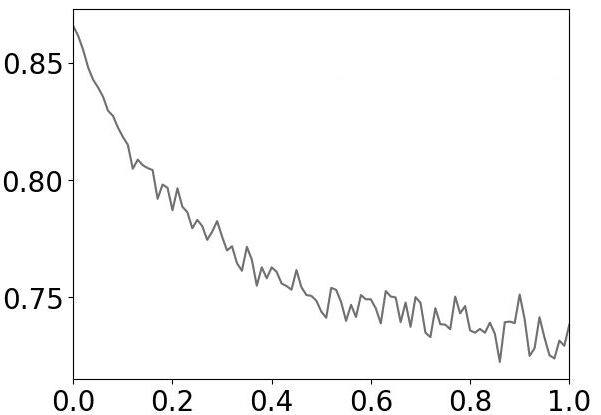
\includegraphics[width=0.48\textwidth]{media/From_IEEE/res_elec_100_h_10_rerun.csv_F1_score_reduced.jpg}
         \label{fig:f1_elec}}
    \subfloat[]{
         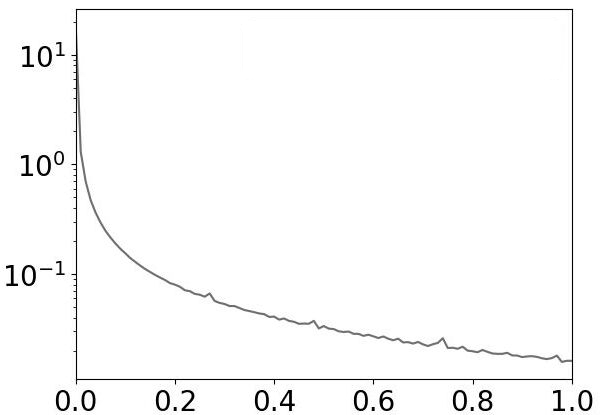
\includegraphics[width=0.48\textwidth]{media/From_IEEE/res_elec_100_h_10_rerun.csv_iter_time_reduced.jpg}
         \label{fig:iter_elec}}
    \\
    \subfloat[]{
         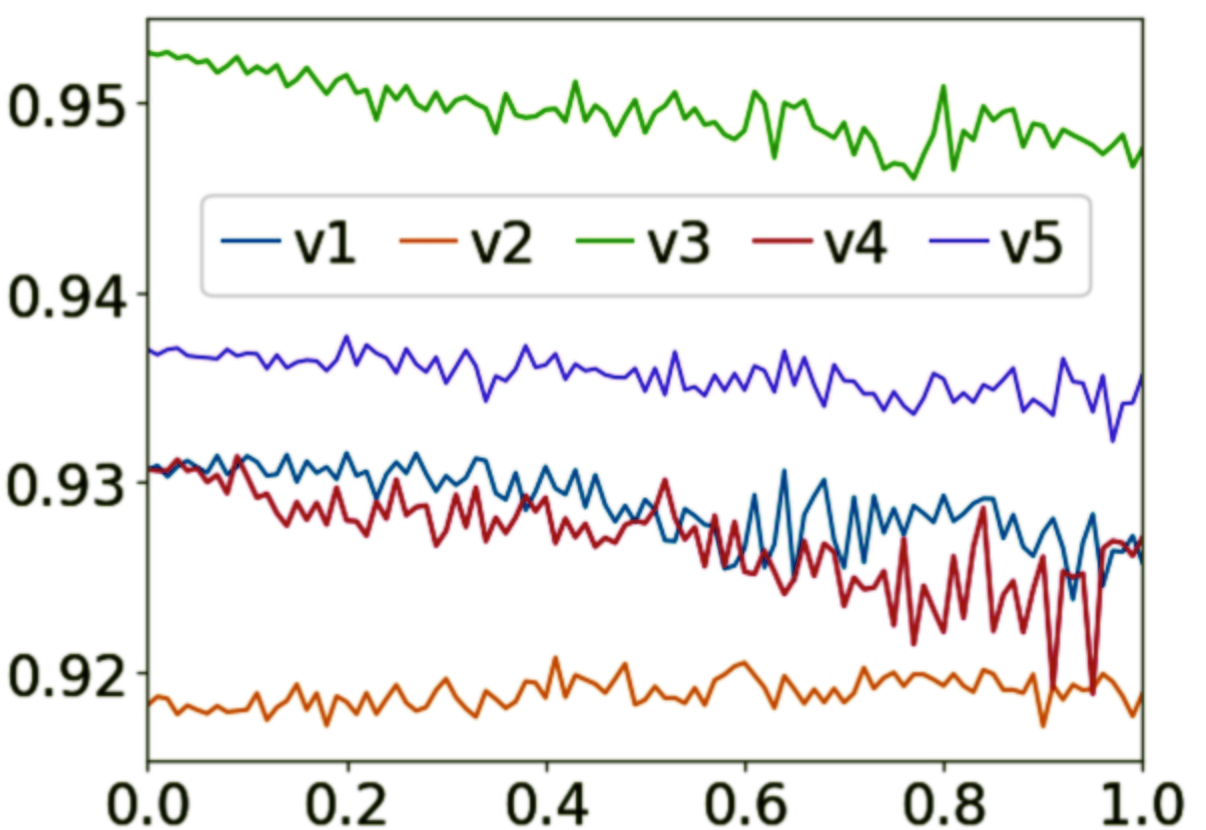
\includegraphics[width=0.48\textwidth]{media/From_IEEE/INSECTS-aggregated_3_F1_score.jpg}
         \label{fig:f1_insects}}
    \subfloat[]{
         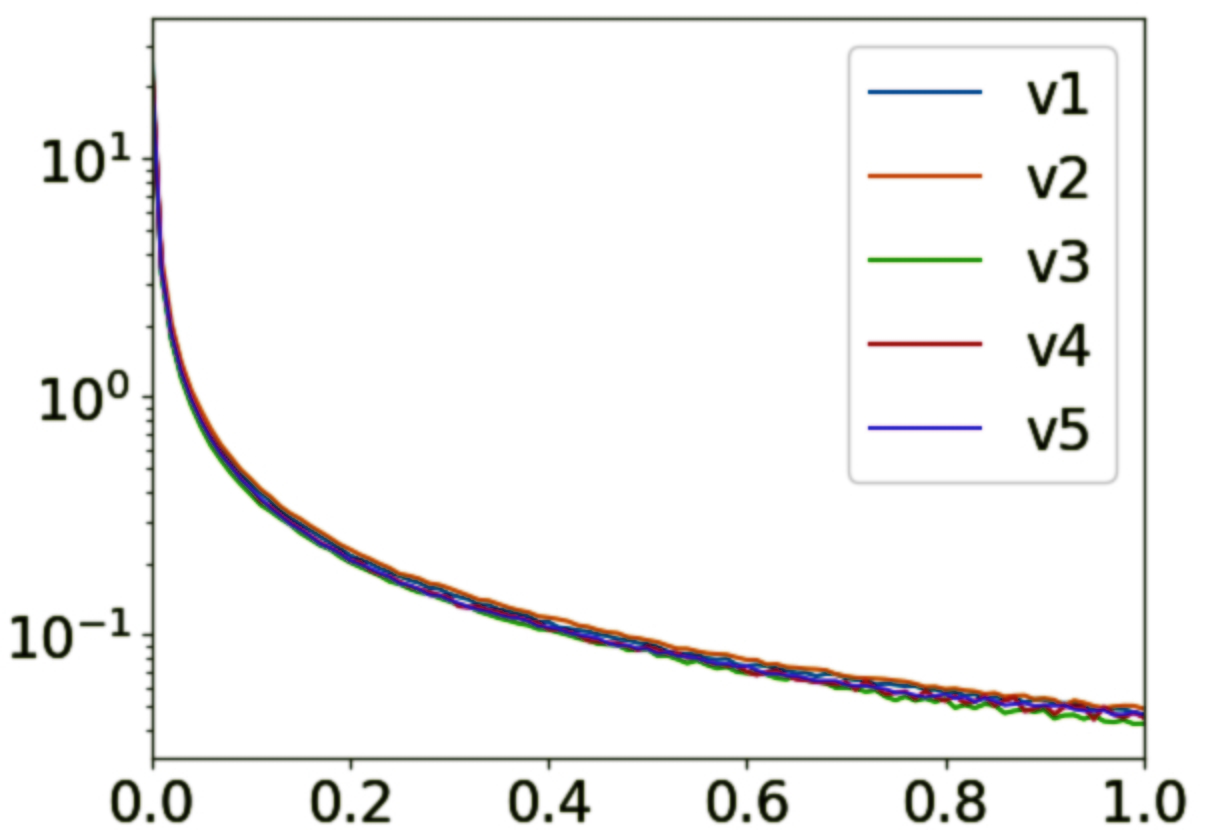
\includegraphics[width=0.48\textwidth]{media/From_IEEE/INSECTS-aggregated_3_iter_time_reduced.jpg}
         \label{fig:iter_insects}}
    \\
    \subfloat[]{
         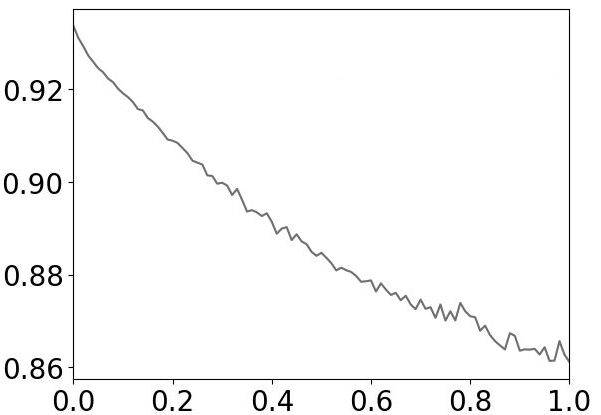
\includegraphics[width=0.48\textwidth]{media/From_IEEE/res_poker-lsn_1000_h_10.csv_F1_score_reduced.jpg}
         \label{fig:f1_poker}}
    \subfloat[]{
         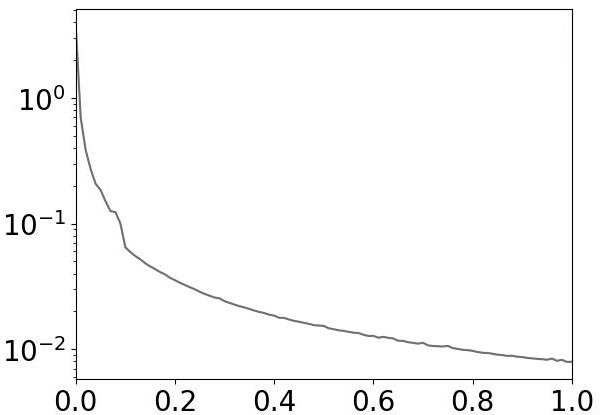
\includegraphics[width=0.48\textwidth]{media/From_IEEE/res_poker-lsn_1000_h_10.csv_iter_time_reduced.jpg}
         \label{fig:iter_poker}}
\caption{Performance of \algo{} in the SW model on the Electricity, INSECTS and Poker datasets (top to bottom), in terms of F1-score (left) and amortized milliseconds per update (right) as a function of $\epsilon$.}\label{fig:SW}
\vspace*{10pt}
\end{figure}

\begin{figure}
\vspace*{10pt}
    \centering
    \subfloat[Electricity]{
         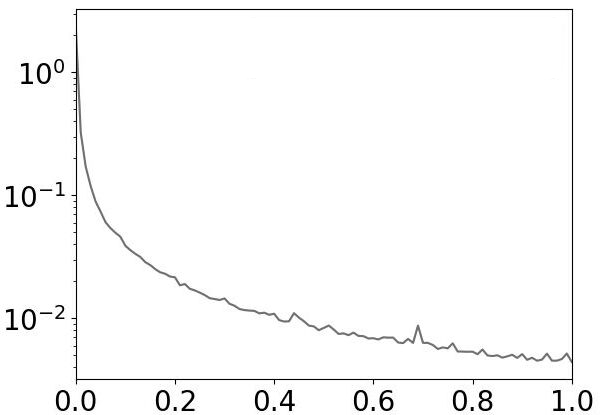
\includegraphics[width=0.48\textwidth]{media/From_IEEE/elec_random.csv_iter_time_reduced.jpg}
         \label{fig:ru_elec}    
    }
    \hfill
    \subfloat[INSECTS]{
         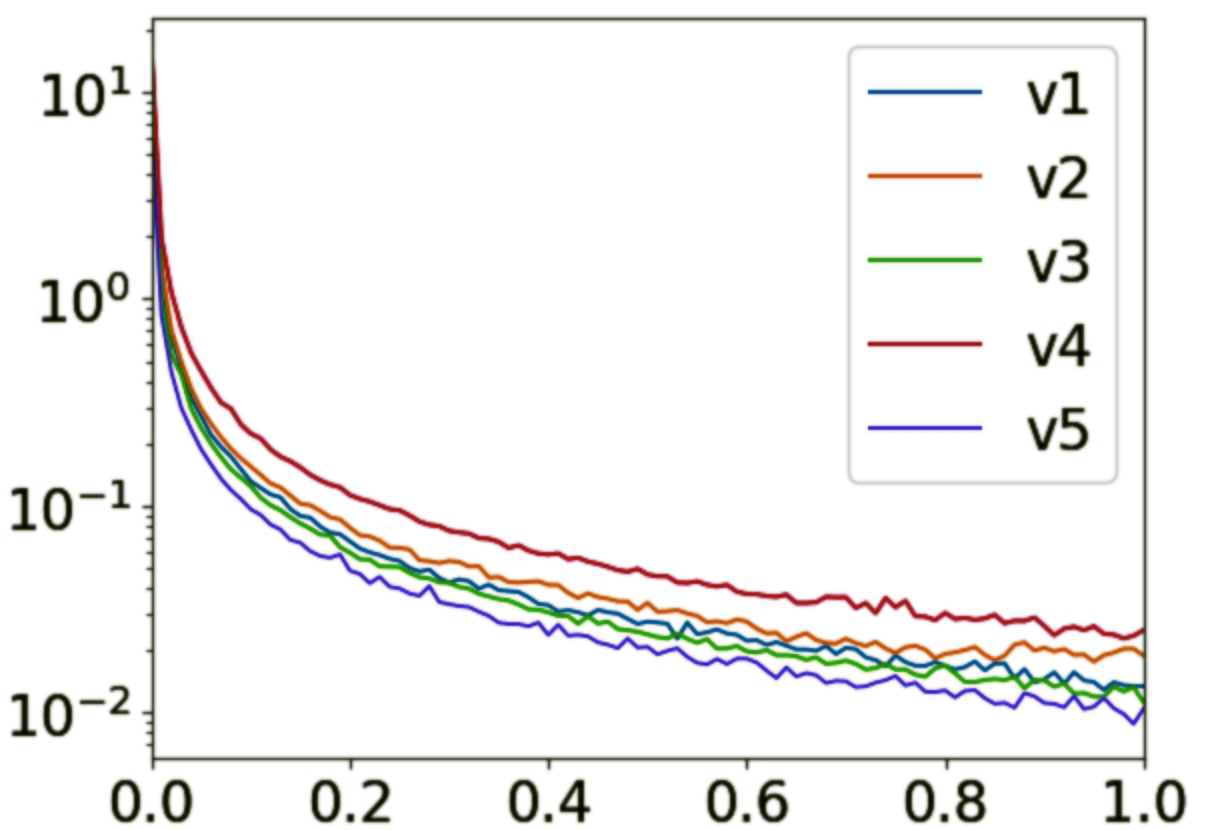
\includegraphics[width=0.48\textwidth]{media/From_IEEE/INSECTS_random-aggregated_3_iter_time_reduced.jpg}
         \label{fig:ru_insects}    
    }
    
    \subfloat[Poker]{
         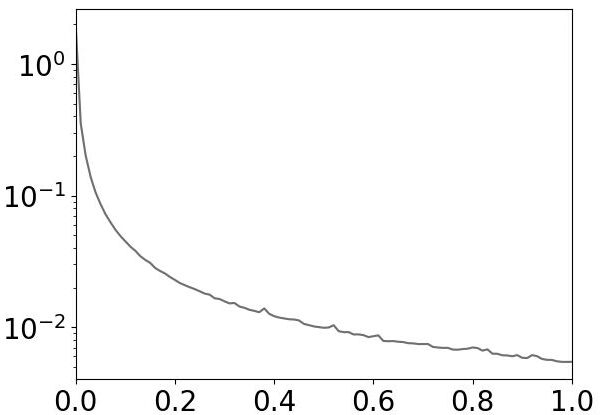
\includegraphics[width=0.48\textwidth]{media/From_IEEE/poker-lsn_random.csv_iter_time_reduced.jpg}
         \label{fig:ru_poker}    
    }
\caption{Amortized running time per update (in milliseconds) of \algo{} in the RU model on the Electricity, Poker and INSECTS datasets.}
\label{fig:RU}
\end{figure}




\iffalse
\begin{figure*}
    \centering
    \subfloat[Electricity (F1-score)]{
         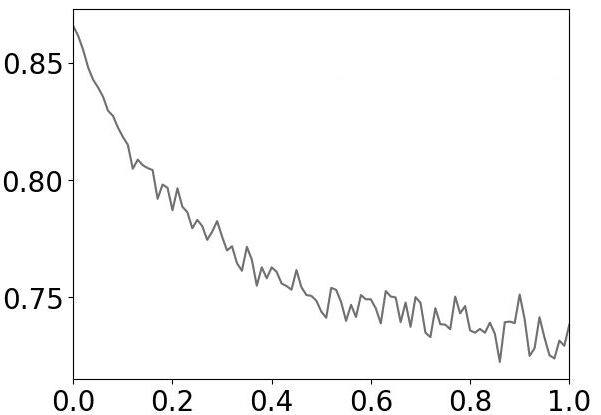
\includegraphics[width=0.3\textwidth]{media/From_IEEE/res_elec_100_h_10_rerun.csv_F1_score_reduced.jpg}
         \label{fig:f1_elec}}
    \hfill
    \subfloat[INSECTS (F1-score)]{
         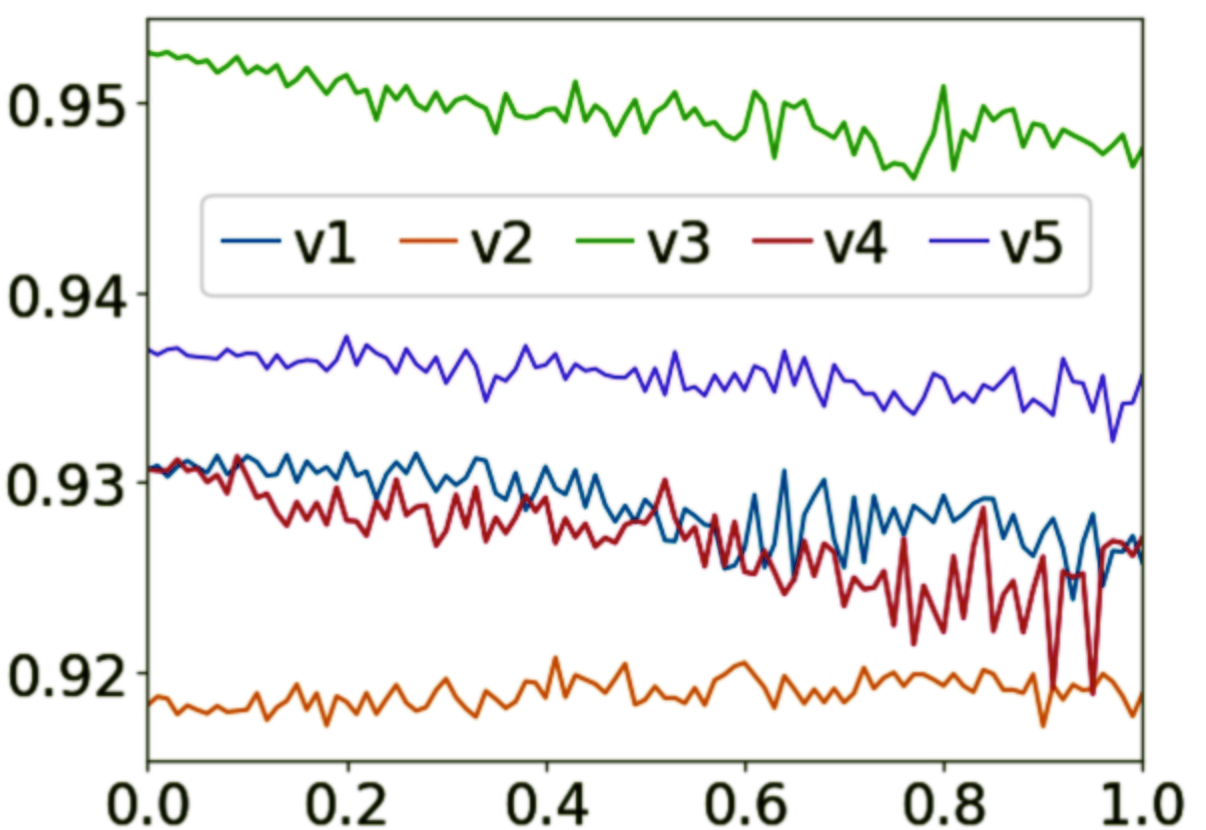
\includegraphics[width=0.28\textwidth]{media/From_IEEE/INSECTS-aggregated_3_F1_score.jpg}
         \label{fig:f1_insects}}
    \hfill
    \subfloat[Poker (F1-score)]{
         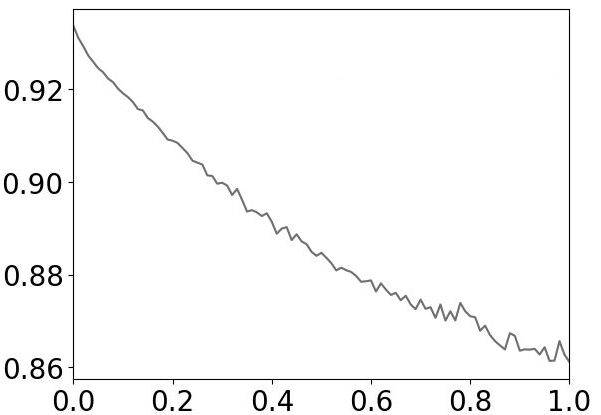
\includegraphics[width=0.3\textwidth]{media/From_IEEE/res_poker-lsn_1000_h_10.csv_F1_score_reduced.jpg}
         \label{fig:f1_poker}    
    }
    \label{fig:f1_scores}
    \subfloat[Electricity (Time)]{
         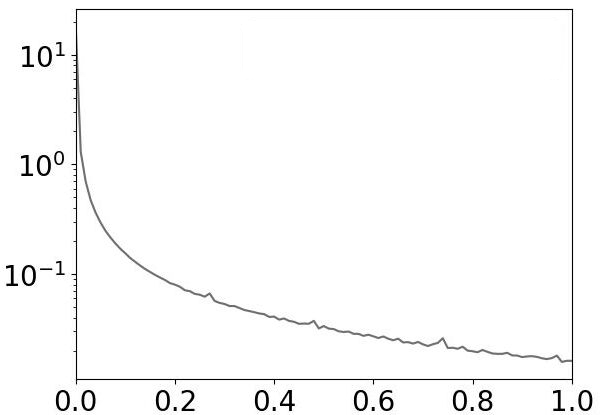
\includegraphics[width=0.3\textwidth]{media/From_IEEE/res_elec_100_h_10_rerun.csv_iter_time_reduced.jpg}
         \label{fig:iter_elec}    
    }
    \hfill
        \subfloat["INSECTS" (Time)]{
         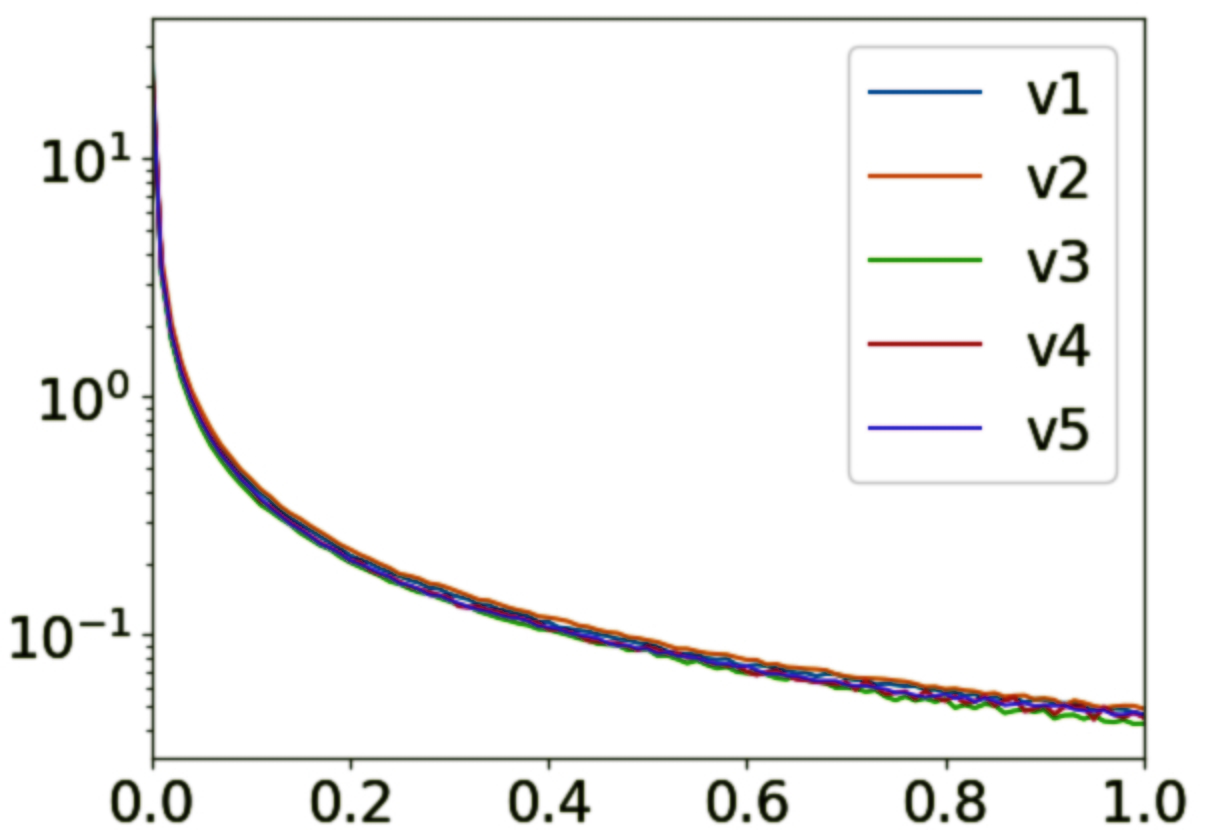
\includegraphics[width=0.28\textwidth]{media/From_IEEE/INSECTS-aggregated_3_iter_time_reduced.jpg}
         \label{fig:iter_insects}    
    }
    \hfill
    \subfloat[Poker (Time)]{
         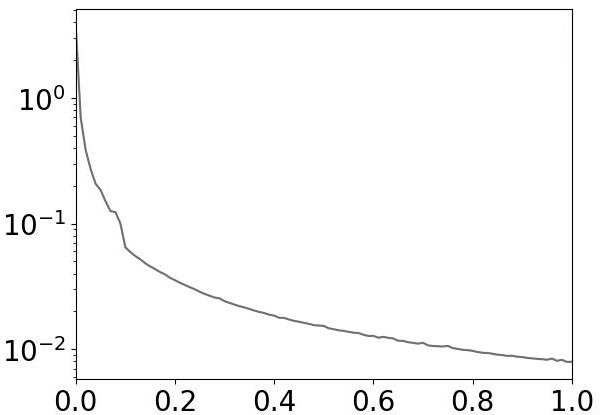
\includegraphics[width=0.3\textwidth]{media/From_IEEE/res_poker-lsn_1000_h_10.csv_iter_time_reduced.jpg}
         \label{fig:iter_poker}    
    }
\caption{F1-score and amortized running time in the SW model.}\label{fig:SW}

\end{figure*}
\fi

\iffalse
\begin{figure*}
    \centering
    \subfloat[Electricity]{
         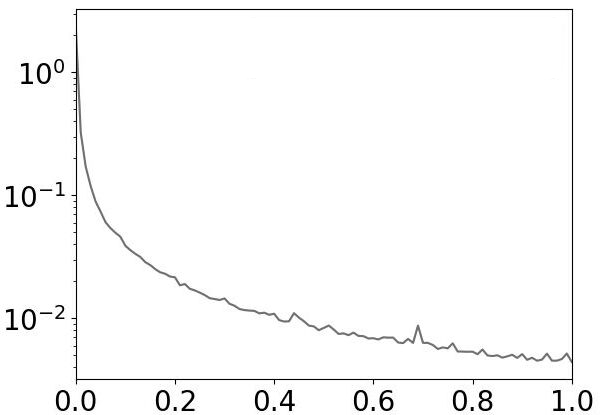
\includegraphics[width=0.3\textwidth]{media/From_IEEE/elec_random.csv_iter_time_reduced.jpg}
         \label{fig:ru_elec}    
    }
    \hfill
    \subfloat[INSECTS]{
         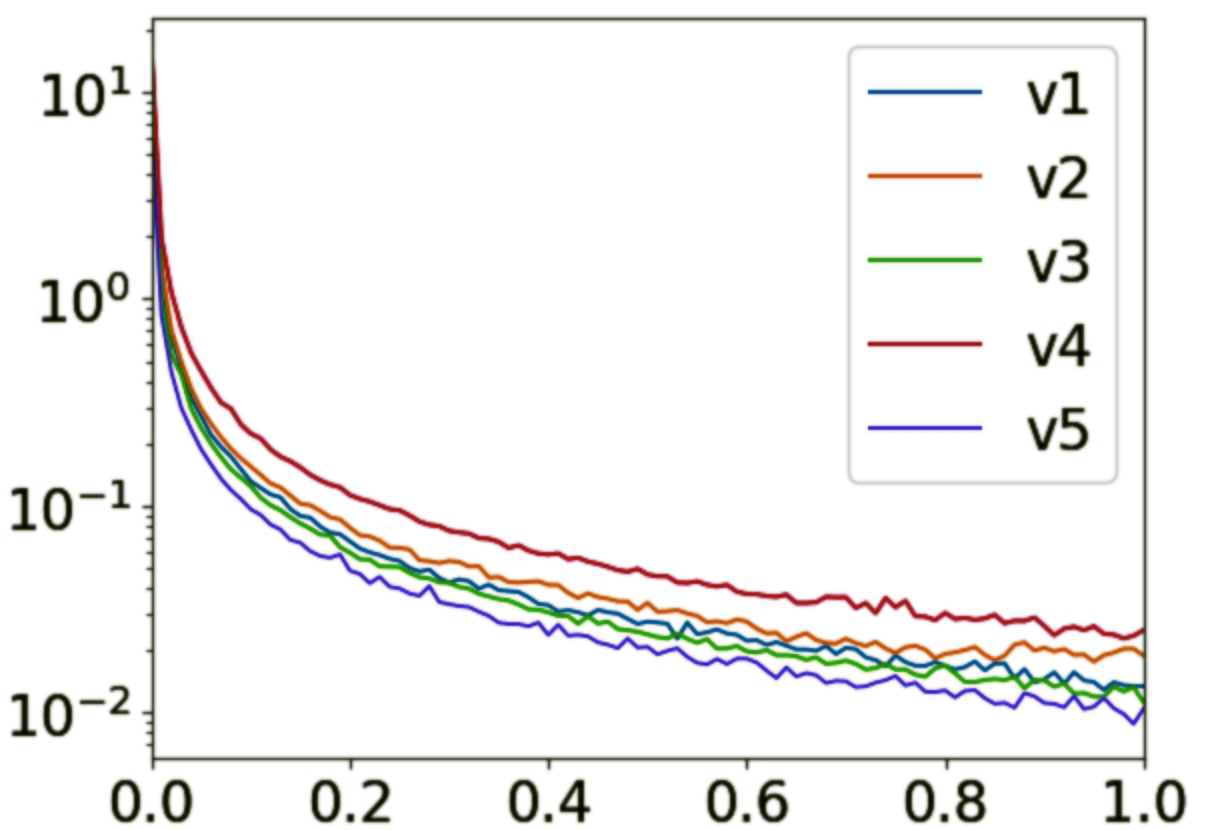
\includegraphics[width=0.28\textwidth]{media/From_IEEE/INSECTS_random-aggregated_3_iter_time_reduced.jpg}
         \label{fig:ru_insects}    
    }
    \hfill
    \subfloat[Poker]{
         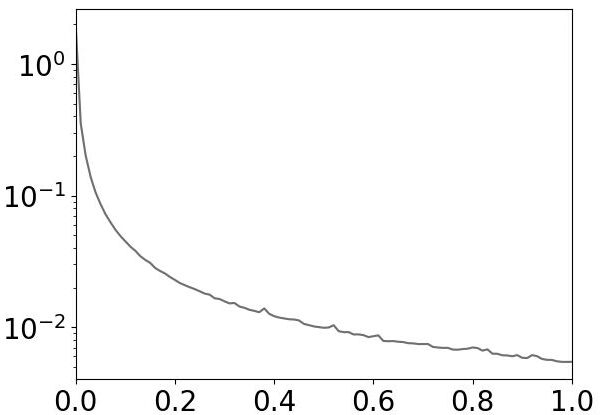
\includegraphics[width=0.3\textwidth]{media/From_IEEE/poker-lsn_random.csv_iter_time_reduced.jpg}
         \label{fig:ru_poker}    
    }
\caption{Amortized running time in the RU model.}\label{fig:RU}
\end{figure*}
\fi

%\iffalse
\subsection{Conclusions and Future Work}
We developed the first fully dynamic algorithm for maintaining $\epsilon$-feasible decision trees, while we proved it to be nearly optimal in terms of space and amortized time. Our work shows that many well-known decision tree algorithms, whether offline like CART or incremental like EFDT, can be made fully dynamic with a small loss in the quality of the decision tree and a small overhead in the amortized running time. Our work leaves open the natural question of whether these results can be strengthened from amortized to worst-case. We believe this is an exciting direction for future research in  fully-dynamic supervised machine learning.
%We developed the first fully dynamic algorithm for maintaining $\epsilon$-feasible decision trees, as well as lower bounds on the space requirements and amortized running time of any such algorithm. Our algorithm boasts near-optimal space requirements and near-optimal running time for some cases of interest. Our experimental evaluation shows that our algorithm is accurate in terms of F1-score, while boasting an average running per update of less than one millisecond. We believe that developing fully-dynamic algorithms for supervised machine learning problems is an exciting research direction that deserves more attention. 
%\fi